\documentclass[reqno,10pt]{amsart}
\usepackage[letterpaper, margin=1in]{geometry}
\RequirePackage{amsmath,amssymb,amsthm,graphicx,mathrsfs,url,slashed,subcaption}
\RequirePackage[usenames,dvipsnames]{xcolor}
\RequirePackage[colorlinks=true,linkcolor=Red,citecolor=Green]{hyperref}
\RequirePackage{amsxtra}
\usepackage{cancel}
\usepackage{tikz-cd}

% \setlength{\textheight}{9.3in} \setlength{\oddsidemargin}{-0.25in}
% \setlength{\evensidemargin}{-0.25in} \setlength{\textwidth}{7in}
% \setlength{\topmargin}{-0.25in} \setlength{\headheight}{0.18in}
% \setlength{\marginparwidth}{1.0in}
% \setlength{\abovedisplayskip}{0.2in}
% \setlength{\belowdisplayskip}{0.2in}
% \setlength{\parskip}{0.05in}
%\renewcommand{\baselinestretch}{1.05}

\title{Functions of least gradient and minimal laminations in constant curvature}
\author{Aidan Backus}
\date{July 2022}

\newcommand{\NN}{\mathbf{N}}
\newcommand{\ZZ}{\mathbf{Z}}
\newcommand{\QQ}{\mathbf{Q}}
\newcommand{\RR}{\mathbf{R}}
\newcommand{\CC}{\mathbf{C}}
\newcommand{\DD}{\mathbf{D}}
\newcommand{\PP}{\mathbf P}
\newcommand{\MM}{\mathbf M}
\newcommand{\II}{\mathbf I}
\newcommand{\Hyp}{\mathbf H}
\newcommand{\Sph}{\mathbf S}
\newcommand{\Group}{\mathbf G}
\newcommand{\GL}{\mathbf{GL}}
\newcommand{\Orth}{\mathbf{O}}
\newcommand{\SpOrth}{\mathbf{SO}}
\newcommand{\Ball}{\mathbf{B}}

\DeclareMathOperator*{\Expect}{\mathbf E}

\DeclareMathOperator{\avg}{avg}
\DeclareMathOperator{\card}{card}
\DeclareMathOperator{\cent}{center}
\DeclareMathOperator{\ch}{ch}
\DeclareMathOperator{\codim}{codim}
\DeclareMathOperator{\Cyl}{Cyl}
\DeclareMathOperator{\diag}{diag}
\DeclareMathOperator{\diam}{diam}
\DeclareMathOperator{\dom}{dom}
\DeclareMathOperator{\Exc}{Exc}
\newcommand{\ext}{\mathrm{ext}}
\DeclareMathOperator{\Gal}{Gal}
\DeclareMathOperator{\Hom}{Hom}
\DeclareMathOperator{\Iso}{Iso}
\DeclareMathOperator{\Jac}{Jac}
\DeclareMathOperator{\Lip}{Lip}
\DeclareMathOperator{\Met}{Met}
\DeclareMathOperator{\id}{id}
\DeclareMathOperator{\rad}{rad}
\DeclareMathOperator{\rank}{rank}
\DeclareMathOperator{\Rm}{Rm}
\DeclareMathOperator{\Hess}{Hess}
\DeclareMathOperator{\Hol}{Hol}
\DeclareMathOperator{\Prop}{Prop}
\DeclareMathOperator{\Radon}{Radon}
\DeclareMathOperator*{\Res}{Res}
\DeclareMathOperator{\sgn}{sgn}
\DeclareMathOperator{\singsupp}{sing~supp}
\DeclareMathOperator{\Spec}{Spec}
\DeclareMathOperator{\supp}{supp}
\DeclareMathOperator{\Tan}{Tan}
\newcommand{\tr}{\operatorname{tr}}

\newcommand{\Mink}{\mathbf m}
\newcommand{\Ric}{\mathrm{Ric}}
\newcommand{\Riem}{\mathrm{Riem}}
\newcommand*\dif{\mathop{}\!\mathrm{d}}
\newcommand*\Dif{\mathop{}\!\mathrm{D}}
\newcommand{\LapQL}{\Delta^{\mathrm{ql}}}

\newcommand{\dbar}{\overline \partial}

\DeclareMathOperator{\atanh}{atanh}
\DeclareMathOperator{\csch}{csch}
\DeclareMathOperator{\sech}{sech}

\DeclareMathOperator{\Div}{div}
\DeclareMathOperator{\Gram}{Gram}
\DeclareMathOperator{\grad}{grad}
\DeclareMathOperator{\dist}{dist}
\DeclareMathOperator{\spn}{span}
\DeclareMathOperator{\Ell}{Ell}
\DeclareMathOperator{\WF}{WF}

\newcommand{\Two}{\mathrm{I\!I}}

\newcommand{\Lagrange}{\mathscr L}
\newcommand{\DirQL}{\mathscr D^{\mathrm{ql}}}
\newcommand{\DirL}{\mathscr D}

\newcommand{\Hilb}{\mathcal H}
\newcommand{\Homology}{\mathrm H}
\newcommand{\normal}{\mathbf n}
\newcommand{\radial}{\mathbf r}
\newcommand{\evect}{\mathbf e}
\newcommand{\vol}{\mathrm{vol}}

\newcommand{\pic}{\vspace{30mm}}
\newcommand{\dfn}[1]{\emph{#1}\index{#1}}

\renewcommand{\Re}{\operatorname{Re}}
\renewcommand{\Im}{\operatorname{Im}}

\newcommand{\loc}{\mathrm{loc}}
\newcommand{\cpt}{\mathrm{cpt}}

\def\Japan#1{\left \langle #1 \right \rangle}

\newtheorem{theorem}{Theorem}[section]
\newtheorem{badtheorem}[theorem]{``Theorem"}
\newtheorem{prop}[theorem]{Proposition}
\newtheorem{lemma}[theorem]{Lemma}
\newtheorem{sublemma}[theorem]{Sublemma}
\newtheorem{proposition}[theorem]{Proposition}
\newtheorem{corollary}[theorem]{Corollary}
\newtheorem{conjecture}[theorem]{Conjecture}
\newtheorem{axiom}[theorem]{Axiom}
\newtheorem{assumption}[theorem]{Assumption}

\newtheorem{mainthm}{Theorem}
\renewcommand{\themainthm}{\Alph{mainthm}}

\newtheorem{claim}{Claim}[theorem]
\renewcommand{\theclaim}{\thetheorem\Alph{claim}}

\theoremstyle{definition}
\newtheorem{definition}[theorem]{Definition}
\newtheorem{remark}[theorem]{Remark}
\newtheorem{example}[theorem]{Example}
\newtheorem{notation}[theorem]{Notation}

\newtheorem{exercise}[theorem]{Discussion topic}
\newtheorem{homework}[theorem]{Homework}
\newtheorem{problem}[theorem]{Problem}

\makeatletter
\newcommand{\proofpart}[2]{%
  \par
  \addvspace{\medskipamount}%
  \noindent\emph{Part #1: #2.}
}
\makeatother

\newtheorem{ack}{Acknowledgements}

\numberwithin{equation}{section}


% Mean
\def\Xint#1{\mathchoice
{\XXint\displaystyle\textstyle{#1}}%
{\XXint\textstyle\scriptstyle{#1}}%
{\XXint\scriptstyle\scriptscriptstyle{#1}}%
{\XXint\scriptscriptstyle\scriptscriptstyle{#1}}%
\!\int}
\def\XXint#1#2#3{{\setbox0=\hbox{$#1{#2#3}{\int}$ }
\vcenter{\hbox{$#2#3$ }}\kern-.6\wd0}}
\def\ddashint{\Xint=}
\def\dashint{\Xint-}

\usepackage[backend=bibtex,style=numeric]{biblatex}
\renewcommand*{\bibfont}{\normalfont\footnotesize}
\addbibresource{topics.bib}
\renewbibmacro{in:}{}
\DeclareFieldFormat{pages}{#1}


\begin{document}
\begin{abstract}
The least-gradient maximum principle, essentially due to Miranda and de Giorgi in the 1960s, shows that least-gradient functions on euclidean space define a minimal lamination of the support of their derivative.
We show that this result holds on manifolds of constant sectional curvature by studying a Plateau-type PDE.
We then apply the least-gradient maximum principle to answer some questions of Daskalopoulos--Uhlenbeck concerning best-Lipschitz maps, generalize a result of G\'orny decomposing least-gradient functions, and propose some future applications.
\end{abstract}

\maketitle

%%%%%%%%%%%%%%%%%%%%%%%%%%%%%%%%%%%%%%%%%%%%%%%%%%%%%%%

% \tableofcontents

\section{Introduction}
Throughout this paper, let $M$ be an oriented Riemannian manifold of metric $g$ and dimension $d$.
For a function $u \in BV_\loc(M)$, we write $\star |\dif u|$ for the total variation of the derivative, c.f. (\ref{total variation}).

\begin{definition}\label{main definitions}
A function $u \in BV_\loc(M)$ has \dfn{least gradient} if for every open $U \Subset M$ and every $v \in BV_\cpt(U)$,
\begin{equation}\label{least gradient functional}
\int_U \star |\dif u| \leq \int_U \star |\dif u + \dif v|.
\end{equation}
A set $U$ of locally finite perimeter has \dfn{least perimeter} if $1_U$ has least gradient.
\end{definition}

Functions of least gradient arise naturally as solutions to an inverse problem in magnetic resonance imaging (MRI) \cite{Nachman2009, Tamasan2019, Joy09} as well as the formal limit of $p$-harmonic functions as $p \to 1$, but we are interested in them primarily because of their application to Thurston's best-Lipschitz maps (see Definition \ref{BestLipDfn}) between closed hyperbolic manifolds \cite{thurston1998minimal}.
An analytic approach to best-Lipschitz maps was introduced by Daskalopoulos--Uhlenbeck \cite{daskalopoulos2020transverse, daskalopoulosPrep1}, where they are viewed as the limit of $p$-harmonic maps as $p \to \infty$, and therefore are ``dual'' in a suitable sense to functions of least gradient.

While we will not need or recall much of the theory of best-Lipschitz maps, we recall that a central topic of interest in their study is their interactions with geodesic laminations:

\begin{definition}
A \dfn{minimal lamination} in $M$ is a partition of a closed subset of $M$ into smooth hypersurfaces, called \dfn{leaves}, with zero mean curvature.
If $M$ is a surface we also call $M$ a \dfn{geodesic lamination}.
\end{definition}

\begin{definition}
Let $\lambda$ be a minimal lamination.
We call $\lambda$ \dfn{discrete} if the moduli space of leaves of $\lambda$ is discrete, and we call $\lambda$ \dfn{analytic} if every leaf of $\lambda$ is analytic.
\end{definition}

The purpose of this paper is to show that functions of least gradient on manifolds $M$ of constant sectional curvature induce minimal laminations in $M$.
This result was already known \cite[Proposition 3.4, Corollary 3.5]{górny2017planar} in the case $M \subseteq \RR^d$, where it was called the \dfn{least-gradient maximum principle}:

\begin{mainthm}[maximum principle]\label{main thm}
Let $2 \leq d \leq 7$ and suppose that $M$ has constant sectional curvature.
Let $u \in BV_\loc(M)$, $A_y := \partial \{u > y\}$, $\lambda := \bigcup_{y \in \RR} A_y$.
Then, if $u$ is a function of least gradient:
\begin{enumerate}
\item $\lambda$ is an analytic minimal lamination in $M$,
\item $A_y$ is either empty or a locally finite union of connected hypersurfaces with boundary, and 
\item if $M$ is the interior of a surface-with-boundary $\overline M$, then $\lambda$ extends to a geodesic lamination of $\overline M$.
\end{enumerate}
Conversely, if $\lambda$ is a discrete minimal lamination, then $u$ has least gradient.
\end{mainthm}

Theorem \ref{main thm} is called a maximum principle because it implies that if $M$ is the interior of a manifold-with-boundary $\overline M = M \cup \partial M$, then the level sets of any function of least gradient on $M$ must extend all the way to the boundary, just as the maximum principle implies that the level sets of the solution to an elliptic Dirichlet problem should behave.
The necessity of the condition $d \leq 7$ is the existence of codimension-$8$ singularities in sets of least perimeter; see \cite[Chapter 11]{Giusti77} for a discussion of that.

The maximum principle is a local statement.
To apply it in a global setting we recall that an affine line bundle $E \to M$ is \dfn{flat with structure group $\RR$} if we have a privileged system of trivializations called \dfn{flat trivializations} such that the transition function $s_{ij}$ takes the form $s_{ij}(y) = y + c_{ij}$ for a constant $c_{ij} \in \RR$.
Thus flat trivializations $u, v$ of the same section satisfy $u = v + c$ on overlaps and the difference of two global sections is a global function.
We sometimes leave the bundle $E$ implicit.

\begin{definition}
Let $u: M \to E$ be a section of an affine line bundle, flat with structure group $\RR$.
We say that $u$ has \dfn{locally least gradient} if every flat trivialization of $u$ has least gradient.
\end{definition}

Since we have not required that the leaves of a minimal hypersurface are globally area-minimizing, the maximum principle also applies to sections with locally least gradient.
We use this fact to generalize a theorem of G\'orny \cite[Theorem 1.2]{górny2017planar}, which decomposes functions of least gradient.

\begin{mainthm}\label{Gorny regularity}
Let $2 \leq d \leq 7$, suppose that $M$ has constant sectional curvature, and let $u: M \to \RR$ have least gradient.
Then there exists an affine line bundle $E \to M$ which is flat with structure group $\RR$, sections $Ju, Cu: M \to E$ of locally least gradient, and a discrete minimal lamination $\lambda$ in $M$, such that:
\begin{enumerate}
\item $Cu$ is continuous,
\item $Ju$ is locally constant on $M \setminus \lambda$,
\item the traces of $Ju$ and $u$ are constant on each side of both leaves of $\lambda$,
\item and $u = Ju - Cu$.
\end{enumerate}
\end{mainthm}

The maximum principle has several applications, including to hyperbolic geometry (discussed in \S\ref{hyperbolicApps}) and possibly to computational geometry (left as an open research direction in \S\ref{open problems}).

% In \S\ref{Global picture}, we associate to every discrete minimal lamination $\lambda$ on a closed space form $M$ a cohomology class $[\lambda] \in H^1(M, \ZZ)$.
% We can combine the maximum principle with a theorem of Loisel \cite{Loisel20} to show that it is possible to recover a minimal lamination from a given cohomology class:

% \begin{mainthm}
% Let $2 \leq d \leq 7$ and suppose that $M$ is a closed space form.
% Then the algorithm of \S\ref{numerics} takes $\xi \in H^1(M, \ZZ)$ as input, returns a discrete minimal lamination $\lambda$ with $[\lambda] = \xi$ as output, and has runtime $\lesssim ?$.
% \end{mainthm}

Let us now discuss the main ingredients in the proof of the maximum principle.
The first is a generalization of Miranda's monotonicity formula \cite[Theorem 2.8]{Miranda66}.
This formula is stronger than monotonicity formulae for minimal surfaces in Riemannian manifolds that we are aware of (e.g. \cite[\S7]{MarquesXX}) in that it gives a lower bound on the rate of growth of the monotone quantity.

\begin{mainthm}[monotonicity formula]\label{monotonicity prestate}
Let $M$ be a Riemannian manifold and $P \in M$. There exists $A \geq 0$ depending continuously on $P$ such that for every function $u$ of least gradient defined near $P$, every exponential normal coordinate system $(x^\mu)$ based at $P$, and $0 < r_1 < r_2 \lesssim 1$,
\begin{align*}
&\left|\int_{r_1}^{r_2} \partial_r \left[r^{1 - d} \int_{B(P, r)} \dif u \wedge \dif x^1 \wedge \cdots \wedge \dif x^{d - 1}\right] \dif r\right|^2 \\
&\qquad \lesssim \left(1 + (d - 1) \log \frac{r_2}{r_1}\right) \left(r_2^{1 - d}\int_{B(P, r_2)} \star |\dif u| \right)\left(\int_{r_1}^{r_2} \partial_r \left[e^{Ar^2} r^{1 - d} \int_{B(P, r)} \star |\dif u|\right] \dif r\right).
\end{align*}
In particular,
\begin{equation}\label{weak monotonicity}
\int_{r_1}^{r_2} \partial_r \left[e^{Ar^2} r^{1 - d} \int_{B(P, r)} \star |\dif u|\right] \dif r \geq 0.
\end{equation}
Moreover, if $M$ is flat or has negative Ricci curvature, then we can take $A = 0$.
\end{mainthm}

We will never use the conclusion about the Ricci curvature, and only include it as a curiosity item.

The monotonicity formula appears in a number of places in the proof of Theorem \ref{main thm}, but its main purpose is to generalize Miranda's proof \cite{Miranda66} of de Giorgi's regularity theorem \cite{deGiorgi61} to manifolds\footnote{\cite{deGiorgi61} is difficult to obtain, as noted by Miranda and Giusti \cite{Miranda66, Giusti77}, so we never directly refer to it.}; we now state this theorem.

\begin{mainthm}[regularity of minimal hypersurfaces]\label{main lma}
Let $2 \leq d \leq 7$ and suppose that $M$ has constant sectional curvature.
Then every set of least perimeter in $M$ is bounded by analytic minimal hypersurfaces.
\end{mainthm}

We refer the reader to the monograph \cite[Part 1]{Giusti77} for a more detailed, English-language exposition of Miranda's argument.
From Theorem \ref{main lma} and general facts about functions of least gradient that appear in \cite{Miranda67}, the proof of Theorem \ref{main thm} is straightforward, and reviewed in \S\ref{Max Princip}.
We prove the regularity theorem by using the monotonicity formula and a Plateau-type equation adapted to manifolds to deduce a generalization, Proposition \ref{de Giorgi}, of the famous de Giorgi lemma to manifolds.

%%%%%%%%%%%%%%%%%%%%%%%%%%%%%%%%%%%%%%%%%%%%%%%

\subsection{Applications to hyperbolic geometry}\label{hyperbolicApps}
Let $M$ be a closed hyperbolic surface.
Daskalopoulos--Uhlenbeck \cite{daskalopoulos2020transverse} considered best-Lipschitz maps $M \to \Sph^1$. They identified a particularly important class of such maps, the $\infty$-harmonic maps, which are particularly significant because they induce geodesic laminations of $M$.

\begin{definition}\label{BestLipDfn}
Write $L_f$ for the Lipschitz constant of a map $f: M \to N$.
A \dfn{best-Lipschitz map} $u: M \to N$ is a minimizer of $L_u$ in a given homotopy class.
For such a map we define the \dfn{maximum-stretch locus}
$$\lambda_u := \{x \in M: L(x) = \sup L\}$$
where $L(x)$ denotes the local Lipschitz constant of $u$ at $x$.
If a best-Lipschitz map $u: M \to \Sph^1$ is the weak limit in $L^r$ for $r > d$ of $p$-harmonic maps as $p \to \infty$, we call $u$ \dfn{$\infty$-harmonic}.
\end{definition}

\begin{theorem}[Daskalopoulos--Uhlenbeck]\label{infinity harmonic laminations}
Suppose that $M$ is a closed hyperbolic surface and $u: M \to \Sph^1$ is $\infty$-harmonic. Then the maximum-stretch locus $\lambda_u$ is a geodesic lamination in $M$.
\end{theorem}

In \cite[\S5]{daskalopoulos2020transverse}, Daskalopoulos--Uhlenbeck prove Theorem \ref{infinity harmonic laminations} by considering the viscosity solution theory of $\infty$-Laplace equation
\begin{equation}\label{infinity laplace}
    \Hess u(\grad u, \grad u) = 0.
\end{equation}
However, the theory of viscosity solutions of (\ref{infinity laplace}) is still nascent, and Daskalopoulos--Uhlenbeck ask \cite[Problem 9.5]{daskalopoulos2020transverse} for a proof of Theorem \ref{infinity harmonic laminations} that bypasses (\ref{infinity laplace}) altogether.

We give a partial resolution of this problem by proving \cite[Theorem-Conjecture 9.6]{daskalopoulos2020transverse}.
Before we state it, we recall from \cite[\S6]{daskalopoulos2020transverse} that to any $\infty$-harmonic map $u: M \to \Sph^1$, one may associate a section $v$ of locally least gradient, which we call a \dfn{Daskalopoulos-Uhlenbeck dual} of $u$, such that (among other properties) $\supp \dif v \subseteq \lambda_u$.
The proof that a Daskalopoulos-Uhlenbeck dual exists does not use Theorem \ref{infinity harmonic laminations}.
Since $\supp \dif v$ is a geodesic lamination, we conclude from the maximum principle that:

\begin{corollary}\label{maximum stretch contains lamination}
The maximum-stretch locus of an $\infty$-harmonic function on a closed hyperbolic surface contains a geodesic lamination.
\end{corollary}

Using the maximum principle one can also show a partial converse to the fact that $\dif v$ endows $\lambda_u$ with the structure of an oriented measured lamination.
For the definitions, see \cite[\S8]{daskalopoulos2020transverse} or \cite{Ruelle75}.
This resolves \cite[Problem 9.7]{daskalopoulos2020transverse}.

\begin{corollary}\label{ruelle sullivan antiderivative}
Let $\lambda$ be an oriented, transversely measured geodesic lamination on a closed hyperbolic surface $M$, and let $\dif v$ be the Ruelle-Sullivan $1$-current induced by $\lambda$.
Then $\dif v$ is the derivative of a section of locally least gradient on $M$.
\end{corollary}
\begin{proof}
As observed in \cite[\S9]{daskalopoulos2020transverse}, if we lift $\dif v$ to a $1$-current $\dif \tilde v$ on the universal cover $\Hyp^2$, then $\dif \tilde v$ is exact and any antiderivative $\tilde v$ of $\dif \tilde v$ has superlevel sets $\{\tilde v \geq y\}$ which are bounded by geodesics.
Moreover we can choose $\tilde v$ to be $\pi_1(M)$-equivariant.
Then the lift $\tilde \lambda$ of the geodesic lamination $\lambda$ to a fundamental domain of $M$ is a geodesic lamination in an open subset of $\Hyp^2$ and so is discrete, owing the chaoticness of the geodesic flow on the cosphere bundle $S'\Hyp^2$.
Thus we obtain a section of least gradient on $M$, by the maximum principle.
\end{proof}

%%%%%%%%%%%%%%%%%%%%%%%%%%%%%%%%%%%%%
\subsection{Some future directions}\label{open problems}
The hypothesis that $M = (M, g)$ has constant sectional curvature is very technically convenient, but it seems probably unnecessary, and with moderately more work, one should be able to remove or significantly weaken it.
A natural starting point would be to prove Theorem \ref{main lma} in the case that $M$ admits a cover by isothermal charts, because in this setting the obvious analogoue of Lemma \ref{Plateau setup lemma} would hold with an identical proof.

A completely different approach to the proof of Theorem \ref{main lma} would be through the phase transition theory. 
To this end, let $W$ be a double-well potential, e.g. $W(x) = (1 - x^2)^2/4$.
If $u^\varepsilon(t)$ is a solution of the Allen-Cahn heat flow
$$\varepsilon^2(\partial_t u^\varepsilon(t) - \Delta u^\varepsilon(t)) + W'(u^\varepsilon(t)) = 0,$$
then the level sets $\{u^\varepsilon = y\}$, $-1 < y < 1$, evolve by an approximate mean curvature flow in the limit $\varepsilon \to 0$ \cite{Guaraco}, and so it is natural to try to approximate $u := 1_U - 1_{U^c}$, where $U$ has least periemter, by solutions $u^\varepsilon$ of the elliptic Allen-Cahn equation $\varepsilon^2 \Delta u^\varepsilon = W'(u^\varepsilon)$.
This approach was used to construct (necessarily unstable) minimal surfaces in threefolds by Chodosh--Mantoulidis \cite{Chodosh_2020}.
The regularity theory already established for the $\varepsilon \to 0$ limit in \cite[Appendix B]{Guaraco} implies that Theorem \ref{main lma} follows from the following:

\begin{conjecture}
Let $u := 1_U - 1_{U^c}$ where $U$ has least perimeter. Then there exists $u^\varepsilon$ solving the elliptic Allen-Cahn equation such that $u^\varepsilon$ has zero Morse index, and the level sets $\{u^\varepsilon = y\}$, $-1 < y < 1$, converge as varifolds as $\varepsilon \to 0$ to $\partial U$.
\end{conjecture}

Of course, the tricky bit is that $u^\varepsilon$ may not, a priori, have zero Morse index.
This approach seems most plausible when $M$ has negative curvature, so as to force the Allen-Cahn energy to have better convexity properties.

As far as the applications to hyperbolic geometry are concerned, a possible lead was suggested in private communication and \cite[Problems 9.12--9.13]{daskalopoulos2020transverse} by Daskalopoulos--Uhlenbeck.
Let $M$ be a closed hyperbolic threefold and $f: M \to \Sph^1$ a fibration; we would like to construct a minimal lamination in $M$ which is compatible with $f$.
By the maximum principle, it suffices to prove the following conjecture:

\begin{conjecture}
Let $M$ be a closed hyperbolic threefold and $f: M \to \Sph^1$ a fibration.
Then there exists a section $v$ of locally least gradient on $M$ such that $[v] = [f]$.
\end{conjecture}

A possible approach to this conjecture is via Daskalopoulos-Uhlenbeck duality.
One would first define a $p$-Laplacian $\Delta_{k,p}$ for $k$-forms on $M$.
Then, given $p \gg 1$ and $\xi \in H^1(M, \RR)$, one would solve the Neumann problem $\Delta_{1, p} u_p = 0$, $[u_p] = \xi$.
By generalizing Daskalopoulos-Uhlenbeck duality, we hope to show the existence of a $q$-harmonic map $v_q$, $1/p + 1/q = 1$, so that $\dif v_q$ is Hodge dual to the $2$-form $\dif u_p$ and satisfies some other nice properties.
Choosing $\xi$ appropriately we obtain $[v_q] = [f]$, and taking the limit $p \to \infty$, we obtain a section $v$ of locally least gradient.
We would then have to show that $\supp \dif v = M$.

It would also be interesting to resolve \cite[Problem 9.5]{daskalopoulos2020transverse}.
By Corollary \ref{maximum stretch contains lamination}, it follows from the following conjecture:

\begin{conjecture}\label{two laminations agree}
Every $\infty$-harmonic function $u$ on a closed hyperbolic surface has a Daskalopoulos-Uhlenbeck dual $v$ such that $\supp \dif v = \lambda_u$.
\end{conjecture}

In the euclidean case, one can also show a well-posedness result \cite[Theorem 1.1]{górny2017planar} using Theorem \ref{Gorny regularity}.
The generalization of this fact is not obvious as we have not extended the Sternberg--Williams--Ziemer theorem \cite{ZiemerWilliamsSternberg1992} to the Riemannian case, so we state it as a conjecture.

\begin{conjecture}
Let $\overline M = M \cup \partial M$ be a compact, strictly convex surface-with-boundary and constant scalar curvature.
Then there exists a solution of the least-gradient Dirichlet problem on $M$ with data in $BV(\partial M)$.
\end{conjecture}

Finally we remark that, thanks to a recent theorem of Loisel \cite{Loisel20}, the maximum principle may have applications in computational geometry.
To be more precise, to compute a minimal surface with prescribed Dirichlet or Neumann conditions, it suffices to find an integer-valued function of least gradient $u$ with the desired boundary data.
This can be arranged, because Loisel's theorem allows for the computation of $u$ using a barrier method in sublinear time. We therefore make the following conjecture:

\begin{conjecture}
Let $\Omega$ be a polytope in $\RR^d$ equipped with a metric of constant sectional curvature, $2 \leq d \leq 7$, let $\mathcal T$ be a quasiuniform triangulation of $\Omega$, and let $S$ be a Lipschitz submanifold $\partial \Omega$ of dimension $d - 2$.
Let $N$ be the minimal hypersurface in $\Omega$ so that $\overline N \cap \partial \Omega S$.
Then if $\mathcal T$ is sufficiently fine depending on $S$, it is possible to compute the set $\{T \in \mathcal T: N \cap T \neq \emptyset\}$ with runtime which is sublinear in $\card \mathcal T$.
\end{conjecture}


%%%%%%%%%%%%%%%%%%%%%%%%%%%%%%%%%%%%%
\subsection{Overview of the paper}
We discuss preliminaries in \S\ref{prelims}: we recall known facts about geometric measure theory on Riemannian manifolds, laminations, and functions of least gradient.

Our next three sections have purely local results:
\begin{itemize}
\item In \S\ref{MollifierSection}, we prove the monotonicity formula, Theorem \ref{monotonicity prestate}, and review its standard consequences.
\item In \S\ref{Plateau section}, we reduce the regularity theorem, Theorem \ref{main lma}, to a de Giorgi-type lemma, Proposition \ref{de Giorgi}, and develop a ``gauge-invariant'' framework for its proof.
\item In \S\ref{proof of De Giorgi}, we prove the de Giorgi lemma using Theorem \ref{monotonicity prestate}.
\end{itemize}

We prove the global results of this paper in \S\ref{GornySec}: we use Theorems \ref{monotonicity prestate} and \ref{main lma} to prove the maximum principle, Theorem \ref{main thm}, and then as a consequence of the maximum principle and a topological argument we conclude the G\'orny decomposition, Theorem \ref{Gorny regularity}.

Finally, in Appendix \ref{geometric computations} we carry out some tedious but elementary computations in $\Hyp^d$ and $\Sph^d$ that we will use in the formulation and proof of the de Giorgi lemma.

%%%%%%%%%%%%%%%%%%%%%%%%%%%%%%%%%%%%%%%%%%%%%%%%

\subsection{Acknowledgements}
I would like to thank Georgios Daskalopoulos, Karen Uhlenbeck, Trent Lucas, Christine Breiner, NSF...


%%%%%%%%%%%%%%%%%%%%%%%%%%%%%%%%%%%%%%%%%%%%%%%%%%
\section{Preliminaries}\label{prelims}
\subsection{Notation and conventions}
For tensor fields we shall use the musical isomorphisms $\sharp, \flat$ and the Einstein convention.
When using the Einstein convention, Greek indices range over $0, 1, \dots$ while Latin indices range over $1, \dots$.
If we have a fixed coordinate system $(x^\mu)$, we sometimes suppress it and write $\partial_\mu := \partial_{x^\mu}$; sometimes we also write $y := x^0$.
The operator $\star$ is the Hodge star, thus $\star 1$ is the Riemannian volume form.
On a submanifold $\Sigma$ of codimension $\geq 1$, $\vol_\Sigma$ denotes the induced volume form and $\star_\Sigma$ denotes the induced Hodge star. We also write $\star_\rho := \star_{B(P, \rho)}$ if $P \in M$ is fixed.
We write $\Japan\xi$ for the Japanese norm $\Japan\xi := \sqrt{1 + |\xi|^2}$
of an element $\xi$ of a normed space.
We write $\int_U \omega \wedge \psi$ for the pairing of a de Rham $\ell$-current $\omega$ with a compactly supported $\ell$-form $\psi$ in an open set $U$.
In particular, we have a Poincar\'e duality map which identifies a $d - \ell$-form $\omega$ with the $\ell$-current $\psi \mapsto \int_U \omega \wedge \psi$.
See \cite{simon1983GMT} for the definition of a de Rham current.
We identify the distributional derivative of a function $u$ with the $d-1$-current
$$\int_U \dif u \wedge \psi = -\int_U u \dif \psi.$$
For a vector field $X$, we write $\star (Xu) := \dif u \wedge \star (X^\flat)$.


%%%%%%%%%%%%%%%%%%%%%%%%%%%%%%%%%%%%%%%%%%%%%%%%%%
\subsection{Riemannian measure theory}
We recall the Riemannian analogue of the main results of \cite[Chapter 1]{Giusti77}.
A function $u$ is in $BV(U)$ iff its derivative $\dif u$ has finite total variation
\begin{equation}\label{total variation}
\int_U \star |\dif u| := \sup_{\substack{||\psi||_{C^0} \leq 1\\\supp \psi \Subset V}} \int_U \dif u \wedge \psi.
\end{equation}
Whether a current has locally finite total variation is independent of the Riemannian metric and so $BV_\loc(M)$ is also independently defined.
By \cite[Theorem 4.14]{simon1983GMT}, for every $u \in BV_\loc(M)$, there exists a $\star |\dif u|$-measurable section $f$ of the cosphere bundle $S'M$ such that for every compactly supported $d-1$-form $\psi$,
\begin{equation}\label{RNy formula}
\int_M \dif u \wedge \psi = \int_M f|\dif u| \wedge \psi.
\end{equation}
The section $f$ of (\ref{RNy formula}) is given pointwise $\star |\dif u|$-almost everywhere, in any local coordinates $(x^\mu)$, by
\begin{equation}\label{Lebesgue point definition}
    f(P) = \left[\lim_{r \to 0} \frac{\int_{B(x, r)} \star \partial_\mu u}{\int_{B(x, r)} \star |\dif u|}\right] ~\dif x^\mu,
\end{equation}
according to the Besicovitch differentiation theorem; here we view $(\dif x^\mu)$ as a basis of $T'_PM$.
Whether the limit $f(P)$ in (\ref{Lebesgue point definition}) exists, or indeed its value as a point of $S'_PM$, denotes not depend on the Riemannian metric or the choice of coordinates.

\begin{definition}
Let $U$ be a set of locally finite perimeter, and let $u = 1_U$. Then:
\begin{enumerate}
\item The \dfn{measure-theoretic boundary} $\partial U$ is the set of points whose Lebesgue density with respect to $M$ is $\in (0, 1)$.
\item The set of points $P$ for which the limit (\ref{Lebesgue point definition}) exists and satisfies $|f(P)| = 1$ is the \dfn{reduced boundary} $\partial^* U$.
\item The $\star |\dif u|$-measurable $1$-form $f$ defined by (\ref{Lebesgue point definition}) is the \dfn{conormal $1$-form} $\normal_U$ to $\partial U$.
\end{enumerate}
\end{definition}

Our definition of reduced boundary and conormal $1$-form follows \cite[Definition 3.3]{Giusti77} and is due to \cite{deGiorgi55}.
See \cite{Battista_2021} for an equivalent definition of reduced boundary on Riemannian manifolds, and see \cite[Chapter 6]{Pugh02} for the definition of Lebesgue density.

\begin{proposition}\label{locality of Caccioppoli}
    Let $U$ be a set of locally finite perimeter with conormal $1$-form $\normal$.
    Then:
    \begin{enumerate}
    \item $\partial^* U$ is either empty or $d-1$-dimensional in the Hausdorff sense, and is $d-1$-rectifiable.
    \item $\partial^* U$ is a dense subset of $\partial U$.
    \item If $\normal$ extends to a continuous $1$-form on $\partial U$, then $\partial^* U = \partial U$ is a $C^1$ hypersurface.
    \item If $\partial^* U = \partial U$ is a $C^1$ hypersurface, then $\normal$ is the conormal $1$-form on $\partial U$ as defined in differential topology, and $\star |\dif 1_U|$ is the induced volume form on $\partial U$.
\end{enumerate}
\end{proposition}
\begin{proof}
Most of the assertions of this proposition are diffeomorphism-invariant, so we may assume that $M = \RR^d$ and appeal to \cite[Chapters 2-4]{Giusti77}.
The proof that $\star |\dif 1_U|$ is the induced volume form is identical to \cite[Example 1.4]{Giusti77}.
\end{proof}

\begin{definition}
Let $M$ be a Riemannian manifold, let $U$ be a set of locally finite perimeter, and let $E$ be a Borel set.
The \dfn{perimeter} of $U$ in $E$ is
$$|E \cap \partial^* U| := \int_E \star |\dif 1_U|.$$
\end{definition}

\begin{proposition}[coarea formula]\label{Coarea2}
Let $M$ be a Riemannian manifold and $u \in BV_\loc(M)$. Then for every open set $E$,
\begin{equation}\label{coarea formula}
\int_E \star |\dif u| = \int_{-\infty}^\infty |E \cap \partial \{u > y\}| \dif y.
\end{equation}
\end{proposition}
\begin{proof}
We follow \cite[Theorem 1.23]{Giusti77}, which first proves (\ref{coarea formula}) for $u \in C^\infty(\RR^d)$ using piecewise linear functions.
Such functions are not available for our purposes; instead we note that if $u \in C^\infty(\RR^d)$ and $u$ has no critical points then (\ref{coarea formula}) follows from Fubini's theorem, the fact that $|E \cap \partial \{u > y\}|$ is the surface area of $E \cap \{u = y\}$ (by Proposition \ref{locality of Caccioppoli}), and the change-of-variables formula.
However the left-hand side of (\ref{coarea formula}) is unaffected by critical points of $u$, and the right-hand side of (\ref{coarea formula}) is unaffected by critical values of $u$ by Sard's theorem.
So (\ref{coarea formula}) holds for $u \in C^\infty(\RR^d)$.

The rest of the proof is identical to \cite[Theorem 1.23]{Giusti77}, so we omit the details.
Taking a sequence in $C^\infty(M)$ that converges to $u$ in $L^1_\loc(M)$\footnote{Recall that $C^\infty(M)$ is not dense in $BV_\loc(M)$.}, and applying Fatou's lemma and the semicontinuity of total variation, we conclude the $\geq$ direction of (\ref{coarea formula}).
Moreover, Stokes' theorem gives that for every $d-1$-form $\psi$ such that $||\psi||_{L^\infty} \leq 1$ and $\supp \psi \Subset E$,
$$\int_E u \wedge \dif \psi = \int_{-\infty}^\infty \int_E |\psi| \star |\dif 1_{\partial \{u > y\}}| \dif y \leq \int_{-\infty}^\infty |E \cap \partial \{u > y\}| \dif y.$$
Taking the supremum over $\psi$ we obtain the direction $\leq$ in (\ref{coarea formula}).
\end{proof}

\begin{proposition}[Miranda trace theorem]\label{traces}
Let $U \subseteq M$ be an open set with nonempty Lipschitz boundary.
For every $u \in BV_\loc(U)$ there exists $v \in L^1_\loc(\partial U)$ such that for every $d-1$-form $\psi$,
\begin{equation}\label{Miranda IBP}
\int_U \dif u \wedge \psi + \int_U u \dif \psi = \int_{\partial U} v\psi.
\end{equation}
Moreover, for almost every $x \in \partial U$,
\begin{equation}\label{convergence of trace}
\int_{U \cap B(x, \varepsilon)} \star |v(x) - u| \ll \varepsilon^d.
\end{equation}
\end{proposition}
\begin{proof}
This follows from a partition-of-unity argument and \cite[Teorema 1]{Miranda67}; we omit the details.
\end{proof}

%%%%%%%%%%%%%%%%%%%%%%%%%%%%%%%%%%%%%%%%%%%%%%%%%%

\subsection{Functions of least gradient}\label{LeastGradientFunctions}
Recall that a function $u \in BV_\loc$ has least gradient iff $u$ is a minimizer of the action $\int_B \star |\dif u|$.
We define
$$\eta(u, U) := \inf_{v \in BV_\cpt(U)} \int_U \star |\dif(u + v)|$$
for $u \in BV_\loc(M)$ and $U \Subset M$, so that $u$ has least gradient iff $\eta(u, U) = \int_U \star |\dif u|$ for every $U$.

Suppose that $u, v \in BV_\loc(M)$ and $U \Subset M$ is bounded by a Lipschitz hypersurface $N$. It is straightforward to generalize \cite[Lemma 5.6]{Giusti77}, thus
\begin{equation}
|\eta(u, U) - \eta(v, U)| \leq ||u - v||_{L^1(N)}. \label{a priori estimate 1}
\end{equation}
In case $v = 0$, we note that by (\ref{convergence of trace}), the trace map is a contraction in $L^\infty$ norm, thus
\begin{equation}
\eta(u, U) \leq ||u||_{L^1(N)} \leq |N| \cdot ||u||_{L^\infty(M)}. \label{a priori estimate 2}
\end{equation}

\begin{definition}
A sequence $(u_n)$ in $BV_\loc(M)$ has \dfn{approximately least gradient} if for every open $U \Subset M$,
$$\limsup_{n \to \infty} \int_U \star |\dif u_n| \leq \liminf_{n \to \infty} \eta(u_n, U) < \infty.$$
\end{definition}

\begin{proposition}[Miranda stability theorem]\label{Miranda convergence}
If a sequence of functions $(u_n)$ has approximately least gradient and $u_n \to u$ in $L^1_\loc(M)$, then $u$ has least gradient, and for every open set $U \Subset M$ with Lipschitz boundary such that $\int_{\partial U} \star |\dif u| = 0$, one has
\begin{equation}\label{convergence in total variation}
\lim_{n \to \infty} \int_U \star |\dif u_n| = \int_U \star |\dif u|.
\end{equation}
\end{proposition}
\begin{proof}
The proof is similar to Teorema 3 and Osservazione 3 in \cite{Miranda67}; we just note the necessary modifications.
Suitable generalizations of Teorema 2 and Osservazione 2 follow from Proposition \ref{traces}.
One needs to add a term of size $o(1)$ to the right-hand side of the inequalities (2.8), (2.9), (2.13), and (2.14); however, in the limit, this term vanishes and so the conclusions (2.15) and (2.16) are unaffected.
\end{proof}

\begin{remark}\label{transversality}
The somewhat unusual condition $\int_{\partial U} \star |\dif u| = 0$ refers to the same Radon measure $\star |\dif u|$ that acts on the open sets of $M$, not on a measure that acts on the relatively open subsets of $\partial U$.
It should be interpreted as a transversality condition: if $u$ is the indicator function of a set $Z$ with $C^\infty$ boundary, then $\int_{\partial U} \star |\dif u| = 0$ if $\partial U$ is transverse to $\partial Z$.
In particular, the notion of convergence in the Miranda stability theorem is weaker than convergence in $BV_\loc(M)$.\footnote{Therefore the Dirichlet problem for functions of least gradient is ill-posed in general, as the trace morphism is discontinuous with respect to the topology for this notion of convergence. See \cite{spradlin2013traces} for an explicit counterexample.}
\end{remark}

\begin{corollary}\label{compactness}
Every sequence $(u_n)$ of approximately least gradient converges in $L^1_\loc$ and almost everywhere along a subsequence to a function of least gradient $u$ such that for every open set $U \Subset M$ of Lipschitz boundary such that $\int_{\partial U} \star |\dif u| = 0$, one has (\ref{convergence in total variation}).
\end{corollary}
\begin{proof}
By compactness of the natural map $BV_\loc \to L^1_\loc$, $(u_n)$ has a convergent subsequence in $L^1_\loc$ and almost everywhere.
The conditions on the limit $u$ follow from the Miranda stability theorem.
\end{proof}

\begin{proposition}\label{level sets are minimal}
For every function $u$ of least gradient, the superlevel sets $\{u > y\}$ have least perimeter.
If we instead have a sequence $(u_n)$ of approximately least gradient, then $(\{u_n > y\})$ has approximately least perimeter.
\end{proposition}
\begin{proof}
In the proof of \cite[Theorem 1]{BOMBIERI1969}, we replace the coarea formula (replace \cite[Theorem 1.6]{Miranda66} with Proposition \ref{Coarea2}) and the Miranda stability theorem (replace \cite[Teorema 3]{Miranda67} with Proposition \ref{Miranda convergence}).
\end{proof}

%%%%%%%%%%%%%%%%%%%%%%%%%%%%%%%%%%%%%%%%%%%%%%%%%%
\subsection{The exponential map}
Let $(M, g)$ be a Riemannian manifold.
Recall that in normal coordinates $(x^\mu)$, we have the expansion
\begin{equation}\label{expand metric}
g_{\mu\nu} = \delta_{\mu\nu} + O(|x|^2)_{\mu\nu}.
\end{equation}
The same estimate holds for the metric on the Poincar\'e ball model of $\Hyp^d$ or the stereographic projection of $\Sph^d$.
One can of course add more terms to this expansion, and in fact we will later use the third-order expansion of the $\sqrt{\det g}$ in normal coordinates \cite[Lemma 3.4]{schoen1994lectures}:
\begin{equation}\label{expand volume form}
\sqrt{\det g} = 1 - \frac{1}{3} \Ric_{\mu\nu}(P) x^\mu x^\nu + O(|x|^3).
\end{equation}
% There is an annoying technicality with normal coordinates: they are not isothermal.\footnote{Suppose that the exponential map is conformal. By checking on planes in the tangent space we may assume that $d = 2$, and hence that $g$ is locally K\"ahler. But every K\"ahler metric with a holomorphic exponential map is flat \cite{MO68766}.} 
% To get around this, we introduce coordinates which are isothermal, but still satisfy the estimate (\ref{expand metric}):

Following \cite{Giusti77}, we often use the freedom to choose coordinates to assume that the normal vectors to certain hypersurfaces $N$ are approximately horizontal
We make this precise by asserting that the conormal $1$-form to $N$, when wedged with the \dfn{vertical $d-1$-form}
\begin{equation}\label{d1 form}
\psi := \dif x^1 \wedge \dif x^2 \wedge \cdots \wedge \dif x^{d - 1}.
\end{equation}
should be close to the volume form.

% \begin{definition}
% We call two coordinate systems $(x^\mu)$ and $(\tilde x^\mu)$, based at $(P, V)$ and $(Q, W)$ respectively, \dfn{compatible} if: TODO update this
% \begin{enumerate}
% \item both $(x^\mu)$ and $(\tilde x^\mu)$ are normal coordinates, or they are both are stereographic coordinates, and 
% \item when written out in the coordinates $(x^\mu)$ and $(\tilde x^\mu)$ respectively, $V$ is a scalar multiple of $W$.
% \end{enumerate}
% \end{definition}

It follows from the definitions and a Taylor expansion that if $(x^\mu)$ and $(\tilde x^\mu)$ are compatible (TODO: redefine this) and based at $P, Q$, and $P, Q \in B_\rho$ for a ball $B_\rho$ of radius $\rho > 0$, then the vertical $d-1$-forms satisfy on $B_\rho$
\begin{equation}\label{compatible verticals}
|\psi - \tilde \psi| \lesssim \rho.
\end{equation}
The same estimate holds on $B_\rho = B(P, \rho)$ if $(x^\mu)$ is stereographic based at $(P, V)$ and $(\tilde x^\mu)$ is normal based at $(P, V)$.

Using (\ref{expand volume form}) for normal coordinates, we study the blowup of $M$ at a point $p$ on the reduced boundary of a set $U$ of least perimeter, giving a generalization of the conjunction of \cite[Theorem 9.3]{Giusti77} and \cite[Theorem 6.2.2]{Simons68}.

\begin{definition}
For a function $u$ on $M$, $P \in M$ we define the \dfn{tangent rescaling} of $u$ at $P$ to be the net of functions $u_t: T_PM \to \RR$, given by
$$u_t(v) = u\left(\exp_P(tv)\right).$$
\end{definition}

\begin{proposition}\label{blowup theorem}
Suppose that $U$ is an open set with least perimeter in $B(P, r)$, $P \in \partial^* U$, and $u = 1_U$.
Furthermore, suppose that $d \leq 7$.
Then the tangent rescaling of $u$ converges as $t \to 0$ along a subsequence (that we also denote $t \to 0$) in $L^1_\loc$ and almost everywhere, to the indicator function $v$ of a half-space $C \subset T_PM$ such that $0 \in \partial C$.
Moreover, for every open set $V \Subset T_PM$ of Lipschitz boundary such that $\partial V$ is transverse to $\partial C$,
$$\lim_{t \to 0} \int_V \star |\dif u_t| = \int_V \star |\dif v|.$$
\end{proposition}
\begin{proof}
We claim that the tangent rescaling $(u_t)$ has approximately least gradient in $T_PM$ (where we give $T_PM$ its euclidean metric). If this true, then by Corollary \ref{compactness}, there exists a set $C$ of least perimeter in $T_PM$, such that the tangent rescaling converges to $v := 1_C$ in the desired sense.
But $T_PM$ is isometric to $\RR^d$, $d \leq 7$, so by the Bernstein--Fleming theorem \cite[Theorem 17.3]{Giusti77}, $\partial C$ is a hyperplane.
The fact that $0 \in \partial C$ follows from the fact that $P \in \partial^* U$.

To prove the claim, write $|\cdot|'$, $\star'$ for the notions taken in the tangent space with its euclidean geometry, and write $U_t$ for the set indicated by $u_t$.
If $V$ is a precompact open subset of $T_PM$, $V_t = \{v \in T_PM: tv \in V\}$, then we have the scale-invariance
\begin{equation}\label{almost blowup scale invariance}
|\partial^* U_t \cap V|' = t^{1 - d}|\partial^* U_1 \cap V_{1/t}|'.
\end{equation}
From (\ref{almost blowup scale invariance}) and the Taylor expansion (\ref{expand volume form}),
$$t^{d - 1} |\partial^* U_t \cap V|' = |\partial^* U_1 \cap V_{1/t}|' \leq e^{O(t^2)} |\partial^* U \cap \exp_P(V_{1/t})|.$$
For every $w \in BV_\cpt(V)$, the least-gradient nature of $u$ gives
$$|\partial^* U \cap \exp_P(V_{1/t})| \leq \int_{(\exp_P)_* V_{1/t}} \star |\dif(u + (\exp_P)_* w_{1/t})| \leq e^{O(t^2)} \int_{V_{1/t}} \star'|\dif(u_1 + w_{1/t})|'.$$
Therefore, after applying (\ref{almost blowup scale invariance}) and (\ref{expand volume form}) again,
$$|\partial^* U_t \cap V|' \leq e^{O(t^2)} t^{1 - d} \int_{V_{1/t}} \star' |\dif (u_1 + w_{1/t})| = e^{O(t^2)} \int_V \star' |\dif (u_t + w)|.$$
Since $V,w$ were arbitrary, we conclude that $(u_t)$ has approximately least gradient.
\end{proof}


%%%%%%%%%%%%%%%%%%%%%%%%%%%%%%

\subsection{Euclidean minimal graphs}
Let us recall some facts about the Plateau equation for minimal hypersurfaces in $\RR^d$.
We remind the reader that $\Japan\xi$ denotes the Japanese norm $\sqrt{1 + |\xi|^2}$.

If $v$ is a function on $\RR^{d - 1}$, then we can use diffeomorphism $x \mapsto (x, v(x))$ to impose coordinates on the graph $N$ of $v$; in these coordinates the metric tensor on $N$ can be easily seen to be $1 + \dif v \otimes \dif v$.
Then by \cite[(24)]{Petersen2008}, the surface area of $N$ in $\Omega \times \RR$ is $\int_\Omega \Japan{\dif v} \dif x$, where $\dif x := \dif x^1 \wedge \cdots \wedge \dif x^{d - 1}$.
The Lagrangian $\Japan{\dif v} \dif x$ is invariant under the scaling
\begin{equation}\label{rescaled solution}
v_\lambda(x) := v(\lambda x)/\lambda.
\end{equation}

As in \cite{deGiorgi61, Miranda66}, de Giorgi's lemma is based on the below key estimate.
To state it, we define for a $1$-form $\xi: \RR^{d - 1} \to (\RR^{d - 1})'$ and $\rho > 0$, the $1$-form $\avg_\rho \xi$ which acts on vectors $v \in T_x\RR^{d - 1} = \RR^{d - 1}$ by
\begin{equation}\label{definition of averaging}
(\avg_\rho \xi(x), v) := \dashint_{B_\rho} (\xi(x), v) \dif x
\end{equation}
where $B_\rho \subset \RR^{d - 1}$.\footnote{(\ref{definition of averaging}) relies on the flatness of the Levi-Civita connection of $\RR^{d - 1}$ to make the identification $T'\RR^{d - 1} = \RR^{d - 1} \times (\RR^{d - 1})'$, so that we cannot replace $\RR^{d - 1}$ with a curved space in this definition.}
Now the below lemma follows from \cite[Lemma 4.2]{Miranda66} and the scale-invariance (\ref{rescaled solution}):

\begin{lemma}[de Giorgi lemma, euclidean minimal graphs]\label{Miranda42 quant}
For every $c_0 > 0$ small there exists $c_1 = c_1(d, c_0) > 0$ such that the following holds.
Let $\beta, \rho > 0$, $0 < \alpha < 1$, $w \in C^1(B_\rho)$, and let $u$ be the harmonic function on $B_\rho$ with $u|\partial B_\rho = w|\partial B_\rho$.
If $||\dif w||_{C^0} \leq c_1$,
\begin{align}
\int_{B_\rho} \Japan{\dif w} - \Japan{\avg_\rho \dif w} \dif x &\leq \beta, \label{Miranda42 hyp} \\
\int_{B_\rho} \Japan{\dif w} - \Japan{\dif u} \dif x &\leq c_1 \beta,
\end{align}
then 
\begin{equation}\label{Miranda42 concl}
\int_{B_{\alpha \rho}} \Japan{\dif w} - \Japan{\avg_{\alpha \rho} \dif w} \dif x \leq (\alpha^{d + 1} + c_0) \beta.
\end{equation}
\end{lemma}

%%%%%%%%%%%%%%%%%%%%%%%%%%%%%%%%%%%%%%%%%%%%%%%%%%%
% \subsection{The global picture} \label{Global picture}
% In applications, we will not be able to apply the maximum principle to globally defined functions of least gradient.
% Instead, we now introduce sections of sheaves which are locally functions of least gradient.



% \begin{definition}
% Let $E \to M$ be an affine line bundle $E \to M$ which is flat with structure group $\RR$.
% A section $u: M \to E$ has \dfn{locally least gradient} if for any flat trivialization $U \subseteq M$ of $E$, $u|U$ becomes a function $U \to \RR$ of least gradient.
% \end{definition}

% We now turn to $\Sph^1$-valued maps of least gradient, which we will use in the applications to hyperbolic and computational geometry.
% Maps $u: M \to \Sph^1$ can be viewed as sections of an affine line bundle, which is flat of structure group $\RR$, by covering $M$ with charts $U$ so that $u|U$ is not surjective, say $\{u = y\} \cap U = \emptyset$, and then identifying $\Sph^1 \setminus \{y\}$ with $(0, 1) \subset \RR$.
% Such charts exist by Theorem \ref{Gorny regularity} if $M$ has constant sectional curvature and dimension $2 \leq d \leq 7$, since they clearly exist if $u$ is continuous or is locally constant away from a set of codimension $\geq 1$.

% \begin{definition}
% Let $M$ have constant sectional curvature and $2 \leq d \leq 7$.
% A map $u: M \to \Sph^1$ has \dfn{least gradient} if, when viewed as a section of an affine line bundle of structure group $\RR$, $u$ has locally least gradient.
% \end{definition}

% Suppose that $M$ is a closed space form and let $\tilde M \to M$ be its universal cover, which we assume to be nontrivial.\footnote{In our applications, we will always assume that $M$ is not simply connected. This is reasonable because if $u: M \to \Sph^1$ is a nonconstant map of least gradient and $M$ is a closed space form with $\pi_1(M) = 0$, then by the maximum principle, there exists a minimal hypersurface $N \subset M$. But by Poincar\'e duality, the homology class $[N] \in H_{d - 1}(M, \RR)$ is zero, which contradicts the fact that $N$ is homologically area-minimizing.}
% Following \cite[\S2]{daskalopoulos2020transverse}, we associate to each map $u: M \to \Sph^1$ a cohomology class $\xi \in H^1(M, \ZZ)$ by letting $\xi$ be the pushforward map in homotopy $u_*: \pi_1(M) \to \pi_1(\Sph^1)$.
% This really is a cohomology class because, by the Hurcewiz theorem and the universal property of the abelianization, we have natural isomorphisms
% $$\Hom(\pi_1(M), \pi_1(\Sph^1)) = \Hom(\pi_1(M), \ZZ) = \Hom(\pi_1(M)^{\mathrm{ab}}, \ZZ) = \Hom(H_1(M, \ZZ), \ZZ) = H^1(M, \ZZ).$$
% In the other direction, for $\xi \in H^1(M, \ZZ)$ we can speak of $\xi$-\dfn{equivariant} functions $\tilde u: \tilde M \to \RR$ on the universal cover: viewing $\xi$ as a map $\pi_1(M) \to \ZZ$, these are the functions $\tilde u$ such that for every $g \in \pi_1(M)$,
% $$\tilde u(gx) = \tilde u(x) + (\xi, g).$$
% If $\xi$ is the cohomology class associated to a map $u: M \to \Sph^1$, then the $\xi$-equivariant functions are exactly those lifts $\tilde v: \tilde M \to \RR$ of maps $v: M \to \Sph^1$ with the same homotopy class as $u$.

% % \begin{proposition}\label{existence of functions of least gradient}
% % Let $M$ be a closed space form. Then for every $\xi \in H^1(M, \ZZ)$ there exists a map of least gradient $u: M \to \Sph^1$ such that $[\dif u] = \xi$.
% % \end{proposition}
% % \begin{proof}
% % For each $p > 1$ there exists a $p$-harmonic map $u_p: M \to \Sph^1$ whose associated cohomology class is $\xi$; this follows from a standard existence argument in the calculus of variations.
% % Then by \cite[Proposition 4.1]{daskalopoulos2020transverse} there exists a subsequence $p \to 1$, a de Rham $1$-current $\psi$, and $\xi$-equivariant function $\tilde u$ so that the Poincar\'e duals of $\dif u_p$ converge to $\psi$ in the weak topology of measures, $\psi$ is Poincar\'e dual to $\xi$, and the Poincar\'e dual of $\dif \tilde u$ is the lift of $\psi$.
% % In particular, by \cite[Theorem 6.10]{daskalopoulos2020transverse}, $\tilde u$ drops to a map $u$ of least gradient.
% % \end{proof}

% TODO: The cohomology class of a discrete minimal lamination

%%%%%%%%%%%%%%%%%%%%%%%%%%%%%%%%%%%%%%%%%%%%%%%%%%%
\section{Monotonicity and mollification}\label{MollifierSection}
We have two purposes in this section: to prove Theorem \ref{monotonicity prestate} and to show that we can approximate minimal perimeters by $C^1$, approximately minimal perimeters.
Fix normal or stereographic coordinates $(x^\mu)$, $\mu = 0, \dots, d - 1$, centered on a point $P \in M$.
We also write $B_r := B(P, r)$.
We use spherical coordinates $(\theta^i)$, $i = 1, \dots, d - 1$, on each sphere $\partial B_r$ which are compatible with $(x^\mu)$ in the sense that $x^0 = f(r) \cos \theta^1$, where $f(r) = r + O_K(r^3)$ if $(x^\mu)$ are stereographic with constant curvature $K$, or $f(r) = r$ if $(x^\mu)$ are normal.
This is possible because
\begin{equation}\label{partial Br is a variety}
\partial B_r = \{(x^0)^2 + \cdots + (x^{d - 1})^2 = f(r)^2\}.
\end{equation}
We write $\dif \sigma$ for the standard measure on $\Sph^{d - 1}$.

\begin{remark}\label{independence of constants}
Let $K$ be a contractible compact set in $M$.
Then all below implied constants may be chosen independently of the choice of $(x^\mu)$ as long as $P \in K$.
This holds because the space of all normal, or stereographic, coordinate systems with basepoint in $K$ is the compact set $K \times \SpOrth_d$. TODO: Simplify this
\end{remark}

%%%%%%%%%%%%%%%%%%%%%%%%%%%%%%%%%
\subsection{Monotonicity formula}
To prepare for the monotonicity formula, we first generalize an estimate that can be isolated from the proof of \cite[Lemma 5.8]{Giusti77}.

\begin{lemma}\label{monotonicity lemma}
Let $u \in C^1(B_R)$, $0 < r_1 < r_2 < R$, and let
$$E(r) = \int_{B_r} \star |\dif u| - \eta(u, r),$$
so that $E(R) = 0$ iff $u$ has least gradient. Then there exists $A \geq 0$ such that for $R > 0$ small,
\begin{equation}\label{monotonicity lemma eqn}
0 \leq \int_{B_{r_2} \setminus B_{r_1}} \star r^{1 - d}\frac{(\partial_ru)^2}{|\dif u|} \leq 2\int_{r_1}^{r_2} \partial_r \left[e^{Ar^2} r^{1-d}\int_{B_r} \star |\dif u|\right] + \frac{O(E(r))}{r^d} \dif r.
\end{equation}
If $g$ has negative Ricci curature or is flat, then $A = 0$.
\end{lemma}
\begin{proof}
We fix $s \in [r_1, r_2]$, work in normal coordinates, and introduce a competitor $v(r, \theta) = u(s, \theta)$.
From the definition of $\eta$,
\begin{equation}\label{consequence of least gradient monotone}
    \eta(u, s) \leq \int_U \star |\dif v| = \int_0^s \int_{\partial B_r} \star_r |\dif v| \dif r.
\end{equation}
Using the expansions (\ref{expand metric}) and (\ref{expand volume form}) in normal coordinates, and applying $\partial_r v = 0$, we obtain the existence of $A \geq 0$ such that
\begin{equation}\label{introduce the ricci tensor}
\int_{\partial B_r} \star_r |\dif v| \leq e^{As^2} \frac{\tilde r^{d - 1}}{s^{d - 1}} \int_{\partial B_s} \star_s |\dif v|.
\end{equation}
Here if $g$ has negative Ricci curvature or is flat, then $A = 0$.
Applying (\ref{consequence of least gradient monotone}) and Fubini's theorem,
\begin{align*}
\eta(u, s) &\leq  e^{As^2} \int_0^s \frac{r^{d - 1}}{s^{d - 1}} \dif r \cdot \int_{\partial B_s} \star_s |\dif v| = \frac{s e^{As^2}}{d} \int_{\partial B_s} \star_s |\dif v|\\
&\leq \frac{s e^{As^2}}{d - 1} \int_{\partial B_s} \star_s |\dif v|.
\end{align*}
By Gauss' lemma, $\dif v$ is the orthogonal projection of $\dif u$ onto $T' \partial B_s$, and its orthocomplement is $\partial_r u$. Therefore by Taylor's theorem,
$$\int_{\partial B_s} \star_s |\dif v| \leq \int_{\partial B_s} \star_s |\dif u| \sqrt{1 - \frac{(\partial_r u)^2}{|\dif u|^2}} \leq \int_{\partial B_s} \star_s \left[|\dif u| - \frac{(\partial_r u)^2}{2 |\dif u|}\right]$$
or in other words
\begin{align*}
\int_{\partial B_s} \star_s \frac{(\partial_r u)^2}{2|\dif u|} &\leq \int_{\partial B_s} \star_s |\dif u| - \frac{d - 1}{s} e^{-As^2} \eta(u, s)\\
&\leq \int_{\partial B_s} \star_s |\dif u| - \frac{d - 1}{s} e^{-As^2} \int_{B_s} \star |\dif u| - O(s^{-1}E(s)).
\end{align*}
We moreover have for $\tilde A \geq 0$ that
$$e^{-\tilde As^2} \partial_s \left[e^{\tilde As^2} s^{1 - d} \int_{B_s} \star |\dif u|\right] = \left[2\tilde As^{2 - d} - \frac{d - 1}{s^d}\right]\int_{B_s} \star |\dif u| + s^{1 - d} \int_{\partial B_s} \star_s |\dif u|$$
so if we choose $\tilde A$ so that
$$-\frac{d - 1}{s} e^{-As^2} = 2\tilde As - \frac{d - 1}{s}$$
then $A = 0$ implies $\tilde A = 0$, and
$$s^{1 - d} \int_{\partial B_s} \star_s |\dif u| - (d - 1)\frac{e^{-As^2}}{s^d} \int_{B_s} \star|\dif u| \leq e^{-As^2} \partial_s\left(e^{As^2} s^{1 - d} \int_{B_s} \star|\dif u|\right).$$
We moreover have $e^{-As^2} \leq 1$, so we can now integrate with respect to $\dif s$ to conclude the result.
\end{proof}

\begin{proof}[Proof of Theorem \ref{monotonicity prestate}]
Let $(x^\mu)$ be normal coordinates, with vertical $d-1$-form $\psi$, and let $u$ have least gradient.
We first compute $\dif u \wedge \psi = \partial_0 u \dif x$
where $\dif x$ is the natural euclidean volume form on $T_PM$.
Moreover, the radial part of $\partial_0$ is $\cos \theta^1$, and $\iota_{\partial_r} \dif x = r^{d - 1} \dif \sigma$.
Thus by (\ref{partial Br is a variety}),
$$\int_{B_r} \dif u \wedge \psi = r^{d - 1}\int_{\partial B_r} u \cos \theta^1 \dif \sigma(\theta)$$
and hence, since $|\cos \theta^1| \leq 1$,
\begin{align}
\left|\int_{r_1}^{r_2} \partial_r \left[r^{1 - d}\int_{B_r} \dif u \wedge \psi\right] \dif r\right|
&= \left|\int_{\Sph^{d - 1}} (u(r_2, \theta) - u(r_1, \theta)) \cos \theta^1 \dif \sigma(\theta)\right| \\
&\leq \int_{\Sph^{d - 1}} |u(r_2, \theta) - u(r_1, \theta)| \dif \sigma(\theta). \label{monotone dump the metric}
\end{align}
The metric $g$ plays no role in (\ref{monotone dump the metric}), so we may use \cite[Lemma 5.3]{Giusti77} to bound
$$\int_{\Sph^{d - 1}} |u(r_2, \theta) - u(r_1, \theta)| \dif \sigma(\theta) \leq \int_{\Sph^{d - 1}} \int_{r_1}^{r_2} r^{1 - d}|\partial_r u(r, \theta)| \dif r \dif\sigma(\theta).$$
To reintroduce the metric we posit that $R$ is small enough that $\dif r \dif \sigma(\theta) \leq \star 2$.
We therefore have
\begin{equation}\label{monotone before cs}
\int_{\Sph^{d - 1}} \int_{r_1}^{r_2} r^{1 - d}|\partial_r u(r, \theta)| \dif r \dif\sigma(\theta) \leq 2 \int_{B_{r_2} \setminus B_{r_1}} \star r^{1 - d}|\partial_r u|
\end{equation}
and if we apply the Cauchy-Schwarz inequality and approximate $u$ by $C^1$ functions (see \cite[pg68]{Giusti77}), it follows from Lemma \ref{monotonicity lemma} that the right-hand side of (\ref{monotone before cs}) is
$$\lesssim \sqrt{\int_{B_{r_2} \setminus B_{r_1}} \star r^{1 - d} |\dif u|} \sqrt{\int_{r_1}^{r_2} \partial_r \left[e^{Ar^2} r^{1-d}\int_{B_r} \star |\dif u|\right] \dif r}.$$
The monotonicity (\ref{weak monotonicity}) follows at once. To strengthen it we just need to bound $r^{1 - d} |\dif u|$.
Integrating by parts,
\begin{align*}
\int_{B_{r_2} \setminus B_{r_1}} r^{1 - d} |\dif u| &= \int_{r_1}^{r_2} r^{1 - d} \partial_r \int_{B_r} \star |\dif u| \dif r \\
&\leq r^{1 - d} \int_{B_r} \star |\dif u| + (d - 1) \int_{r_1}^{r_2} r^{-d} \int_{B_r} \star |\dif u| \dif r.
\end{align*}
Using (\ref{weak monotonicity}) we bound this second integral as
\begin{align*}
\int_{r_1}^{r_2} r^{-d} \int_{B_r} \star |\dif u| \dif r &\leq r^{1 - d} \log \frac{r_2}{r_1} \int_{B_{r_2}} \star |\dif u|. \qedhere
\end{align*}
\end{proof}

We now control the surface area of a minimal perimeter, generalizing \cite[Remark 5.13]{Giusti77}.
This gives a quantitative sense in which a minimal perimeter has codimension $1$.
Write $\Ball^\ell$ for the unit ball in $\RR^\ell$.

\begin{lemma}\label{least perimeter minimal size}
For a set $U$ of least perimeter, if $P \in \partial^* U$ and $d \leq 7$, one has
$$\lim_{r \to 0} r^{1 - d} |\partial^* U \cap B(P, r)| = |\Ball^{d - 1}|.$$
\end{lemma}
\begin{proof}
Choose a sequence of $r \to 0$; then there is a subsequence along which the limit in Proposition \ref{blowup theorem} exists for $u = 1_U$.
With notation as in the proof of Proposition \ref{blowup theorem},
$$r^{1 - d} |\partial^* U \cap B(P, r)| = e^{O(r^2)} r^{1 - d}\int_{B'_r} \star'|\dif u_1|' = e^{O(r^2)} \int_{B'_1} \star'|\dif u_r|'.$$
Then $u_r \to 1_C$ for $C$ a half-space, which in particular is transverse to $B'_1$.
So by the Miranda stability theorem and Remark \ref{transversality},
\begin{align*}
\lim_{r \to 0} e^{O(r^2)} \int_{B'_1} \star'|\dif u_r|' &= \int_{B'_1} \star'|\dif 1_C|' = |\partial C \cap B'_1|' = |\Ball^{d - 1}|. \qedhere
\end{align*}
\end{proof}

\begin{proposition}[surface area estimate]\label{doubling dimension}
If $d \leq 7$ then there exists $A \geq 0$ such that for every set $U$ of least perimeter in a ball $B_r = B(P, r)$, with $P \in \partial^* U$, and $r > 0$ small,
$$|\Ball^{d - 1}|e^{-Ar^2}r^{d - 1} \leq |\partial^*U \cap B_r| \leq |\Sph^{d - 1}|e^{Ar^2} r^{d - 1}.$$
\end{proposition}
\begin{proof}
The upper bound on $|\partial^* U \cap B_r|$ is obtained by using (\ref{a priori estimate 2}) and the fact that the surface area of $\partial B_r$ is $|\Sph^{d - 1}|(1 + O(r^2))r^{d - 1}$.
This can be seen by integrating $\star_{\partial B_r} 1$ along $\partial B_r$ in normal coordinates and applying (\ref{expand volume form}).
The lower bound is obtained from the monotonicity formula, which implies that
$$\lim_{\rho \to 0} e^{-A\rho^2} \rho^{1 - d} |\partial^* U \cap B_\rho| \leq |\partial^* U \cap B_r|.$$
The left-hand side is given by Lemma \ref{least perimeter minimal size}.
\end{proof}

%%%%%%%%%%%%%%%%%%%%%%%%%%%%%%%%%%%%%%%%%%%%%%%%%%%%%%%%%%%%%%%%
\subsection{Mollification of sets of least perimeter}
Our goal for this section is to generalize \cite[Lemma 7.5]{Giusti77}, which reduces the study of sets of least perimeter to that of sets with $C^1$ perimeter.

In this section, we work with either normal or stereographic coordinates $(x^\mu)$.
The convolution $f * g$ of two functions defined near $P$, or the subtraction $x - y$ of two points near $P$, are meant in the sense of the coordinates $(x^\mu)$\footnote{and crucially, not in terms of the coordinates $(\tilde x^\mu)$ that we introduce in the proof of Lemma \ref{mollifier sublemma}} and the volume form $\dif x := \dif x^0 \wedge \cdots \wedge \dif x^{d - 1}$ obtained from them. Following \cite[Chapter 7]{Giusti77} we define the convolution kernel
$$\chi_\varepsilon(x) := \frac{d + 1}{|\Ball^d|} \varepsilon^{-d}1_{|x| < \varepsilon} \left(1 - \frac{|x|}{\varepsilon}\right)$$
For this section only, we write $u_\varepsilon := u * \chi_\varepsilon$ whenever $u \in BV$ is defined near $P$.

Our first goal is to prove a Riemannian analogue of \cite[Theorem 7.3]{Giusti77}, which estimates $(1_U)_\varepsilon$ for $U$ a set of least perimeter.
The argument there required one to cover $\partial^* U$ by small balls and apply the monotonicity formula in each ball.
To deal with the somewhat large number of parameters involved here, it may helpful to think of the case $\Delta = 1$, in which case we have
$$1 \gg \gamma^q \gg \sigma \gg \gamma \gg \varepsilon \gg \varepsilon \delta > 0.$$

\begin{lemma}[control on $u_\varepsilon$ in each ball]\label{mollifier sublemma}
Let $q < \min(1/8, 1/(4(d - 1)))$.
For every $0 < \Delta, \gamma \lesssim 1$, if we let $\varepsilon = \gamma^4 \Delta$, $\sigma = \gamma^{1/(2(d - 1))} \Delta$, $\delta = \gamma^d$, and let $u$ be the indicator function of a set $U$ of least perimeter such that
\begin{equation}\label{hypothesis on mollifier sublemma}
\int_{B_\Delta} \star(|\psi| \cdot |\dif u| - \dif u \wedge \psi) \leq \Delta^{d - 1} \gamma,
\end{equation}
then on $B_{\Delta - 2\sigma}$, if $Q \in \partial^* U$,
$$(1_{B(Q, 2\delta\varepsilon)}(|\psi| \cdot |\dif u| - \star(\dif u \wedge \psi)))_\varepsilon \ll \gamma^q (1_{B(Q, \delta\varepsilon)} |\dif u|)_\varepsilon.$$
\end{lemma}
\begin{proof}
We first claim that for $r > 0$ so small that $B(Q, 2r) \subseteq B_\varepsilon$,
\begin{equation}\label{bound the kernel}
\sup_{y \in B(Q, 2r)} \chi_\varepsilon(x - y) \lesssim \inf_{y \in B(Q, r)} \chi_\varepsilon(x - y).
\end{equation}
In the euclidean case (with constant equal to $4$) this result can be isolated from the proof of \cite[Theorem 7.3]{Giusti77}.
Otherwise, we can use the smallness of $\varepsilon$ and the expansion (\ref{expand metric}) to approximate $g$-balls by euclidean balls.
This suffices to prove (\ref{bound the kernel}), since $\chi_\varepsilon$ is uniformly continuous.

Now let $V := B(Q, 2\delta\varepsilon)$.
Integrating (\ref{bound the kernel}) against $1_V(|\psi| \cdot |\dif u| - \star(\dif u \wedge \psi))$,
\begin{equation}\label{kernel bounded}
(1_V(|\psi| \cdot |\dif u| - \star(\dif u \wedge \psi)))_\varepsilon(x) \lesssim \inf_{y \in B(Q, \delta\varepsilon)} \chi_\varepsilon(x - y) \int_V \star |\psi| \cdot |\dif u| - \dif u \wedge \psi.
\end{equation}
To estimate the right-hand side of (\ref{kernel bounded}) we introduce a new coordinate system $(\tilde x^\mu)$ of coordinates based at $Q$ which are compatible with $(x^\mu)$.
We write $\tilde g$ for the metric written in these new coordinates, and write $\tilde \psi$ for their vertical $d-1$-form.
By (\ref{compatible verticals}),
\begin{equation}\label{split up T Ttilde}
\int_V \star |\psi| \cdot |\dif u| - \dif u \wedge \psi \leq \int_V \star |\psi| \cdot |\dif u| - \dif u \wedge \tilde \psi + O(\varepsilon) \int_V \star |\dif u|.
\end{equation}
The error term here is given by Proposition \ref{doubling dimension} and the assumption $\Delta \lesssim 1$ as $\lesssim \gamma^2 \int_{B(Q, \delta\varepsilon)} \star |\dif u|$.
To estimate the dominant term in (\ref{split up T Ttilde}) we assume that $\gamma$ is chosen so small that $\sigma > 2\delta\varepsilon$, so that if we set $W := B(Q, \sigma)$ and apply the monotonicity formula and (\ref{compatible verticals}) to obtain $A \geq 0$ such that
\begin{align*}
(2\delta\varepsilon)^{1 - d} &\int_V \star |\psi| \cdot |\dif u| - \dif u \wedge \psi \\
&\leq \sigma^{1 - d}\int_W \star |\dif u| + (2\delta\varepsilon)^{1 - d} \int_V \star(|\psi| - 1)|\dif u| + 2A\sigma^{3 - d} \int_W \star |\dif u| - (2\delta\varepsilon)^{1 - d}\int_V \dif u \wedge \psi\\
&\leq \sigma^{1 - d}\int_W \star |\dif u| - \dif u \wedge \psi + (2\delta\varepsilon)^{1 - d} \int_V \star(|\psi| - 1)|\dif u| + 2A\sigma^{3 - d} \int_W \star |\dif u| \\
&\qquad + O(\varepsilon \sigma^{1 - d}) \int_W \star |\dif u| + \sigma^{1 - d}\int_W \dif u \wedge \tilde \psi - (2\delta\varepsilon)^{1 - d}\int_V \dif u \wedge \tilde \psi\\
&=: I_1 + I_2 + I_3 + I_4 + I_5 - I_6.
\end{align*}
We apply (\ref{hypothesis on mollifier sublemma}) to bound $I_1 \leq \gamma^{1/2}$, and we use the Taylor expansion of the metric on $V$ to bound $|\psi| - 1 \lesssim \varepsilon^2$ on $B_\varepsilon$.
By Proposition \ref{doubling dimension} and the assumption $\Delta \lesssim 1$, it follows that $I_2 + I_3 + I_4 \lesssim \gamma^{1/(d - 1)}$.

To estimate $I_5 - I_6$, we apply the monotonicity formula, using (\ref{compatible verticals}) to replace the $d-1$-form $\tilde \psi$ with the vertical $d-1$-form associated to normal (rather than stereographic) coordinates, if necessary:
\begin{align*}
&\sigma^{1 - d} \int_W \dif u \wedge \tilde \psi - (2\delta\varepsilon)^{1 - d} \int_V \dif u \wedge \tilde \psi \\
&\qquad \lesssim \sqrt{1 + (d - 1) \log \frac{\sigma}{2\delta\varepsilon}} \sqrt{\sigma^{1 - d} \int_W \star |\dif u|} \sqrt{\int_{2\delta\varepsilon}^\sigma \partial_r \left[e^{Ar^2} r^{1 - d} \int_{B(Q, r)} \star |\dif u|\right] \dif r}\\
&\qquad \qquad + \varepsilon \sigma^{1 - d} \int_W \star |\dif u| + \varepsilon (2\delta\varepsilon)^{1 - d} \int_V \star |\dif u| \\
&\qquad =: J_1 J_2 J_3 + J_4 + J_5.
\end{align*}
We have $J_1 \lesssim -\log \gamma$, from Proposition \ref{doubling dimension} we have $J_2 \lesssim 1$, and finally $J_4 + J_5 \lesssim \gamma^4$.
So, we need to get a gain from $J_3$, which we do as follows:
\begin{align*}
J_3^2 &\leq \sigma^{1 - d} \int_W \star |\dif u| - (2 \delta \varepsilon)^{1 - d} \int_V \star |\dif u| + 2A\sigma^{3 - d} \int_W \star |\dif u| \\
&= \sigma^{1 - d} \int_W \star |\dif u| - \dif u \wedge \psi + \sigma^{1 - d} \int_W \dif u \wedge (\psi - \tilde \psi) + \sigma^{1 - d} \int_W \dif u \wedge \tilde \psi \\
&\qquad - (2 \delta\varepsilon)^{1 - d} \int_V \star |\dif u| + 2A \sigma^{3 - d} \int_W \star |\dif u| \\
&=: K_1 + K_2 + K_3 - K_4 + K_5.
\end{align*}
Then $K_1 = I_1 \leq \gamma^{1/2}$, $K_2 \lesssim I_3 \lesssim \gamma^4$, and $K_5 = I_2 \lesssim \gamma^{1/(d - 1)}$.

To estimate $K_3 - K_4$ we observe that for $u = 1_U$,
\begin{equation}\label{K3 calculus}
K_3 = \sigma^{1 - d} \int_W \dif u \wedge \tilde \psi = \sigma^{1 - d} \int_{U \cap \partial W} \tilde \psi.
\end{equation}
We decompose
$$\partial W = \Gamma_+ \cup \Gamma_0 \cup \Gamma_-$$
where $\tilde x^0 > 0$ on $\Gamma_+$ and $\tilde x^0 < 0$ on $\Gamma_-$. Then all positive contributions to the integral in the right-hand side of (\ref{K3 calculus}) come from $\Gamma_+$.
Moreover, as $d-1$-cells in $M$, $\partial \Gamma_+ = \Gamma_0$, but also if we set $N = \{\tilde x^0 = 0\}$ and $W_0 = W \cap N$, then $\Gamma_0 = \partial W_0$.
In particular, there is a homotopy relating $\Gamma_+$ and $\partial W_0$ which holds $\Gamma_0$ fixed.
Since $\dif \psi = 0$, we can use (\ref{partial Br is a variety}) as follows:
\begin{align*}
K_3 &\leq \sigma^{1 - d} \int_{\Gamma_+} \tilde \psi = \sigma^{1 - d} \int_{W_0} \tilde \psi \leq |\Ball^{d - 1}| + O(\sigma^2).
\end{align*}
Hence by Proposition \ref{doubling dimension},
$$K_3 \leq |\Ball^{d - 1}| + O(\sigma^2) \leq K_4 e^{O(\varepsilon\delta)^2} + O(\sigma^2) \leq K_4 + O(\sigma^2) \leq K_4 + O(\gamma^{1/(d - 1)}).$$
In conclusion, $J_3 \lesssim \gamma^{\min(1/4, 1/(d - 1))}$, and hence by (\ref{kernel bounded}) we have for some $q > 0$ that
$$(1_V(|\dif u| - \star(\dif u \wedge \psi)))_\varepsilon(x) \ll (\delta\varepsilon)^{d - 1} \gamma^q \inf_{y \in B(Q, \delta\varepsilon)} \chi_\varepsilon(x - y).$$
Finally, by Proposition \ref{doubling dimension},
\begin{align*}
(\delta\varepsilon)^{d - 1} \inf_{y \in B(Q, \delta\varepsilon)} \chi_\varepsilon(x - y) &\lesssim (1_{B(Q, \delta\varepsilon)} |\dif u|)_\varepsilon(x). \qedhere
\end{align*}
\end{proof}

\begin{figure}
\centering
\begin{subfigure}[b]{0.4\linewidth}
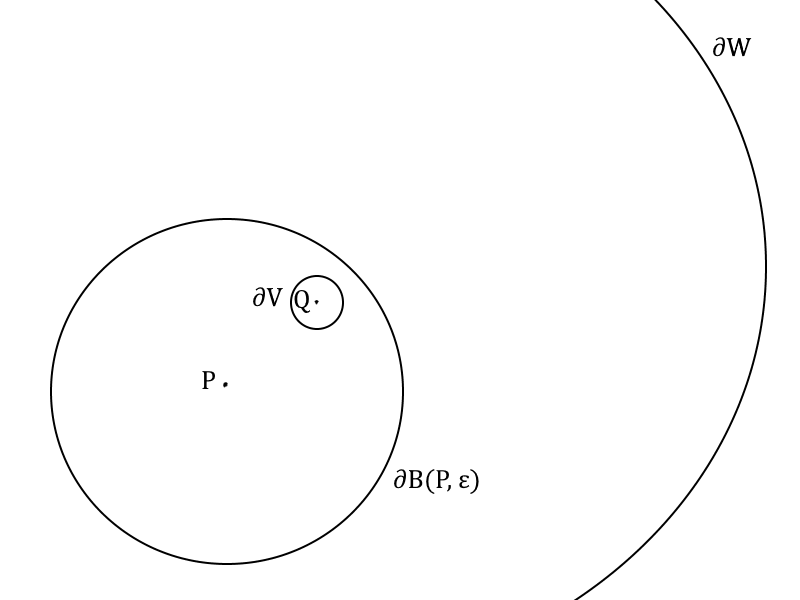
\includegraphics[width=\linewidth]{estimating_scales.png}
\end{subfigure}
\begin{subfigure}[b]{0.4\linewidth}
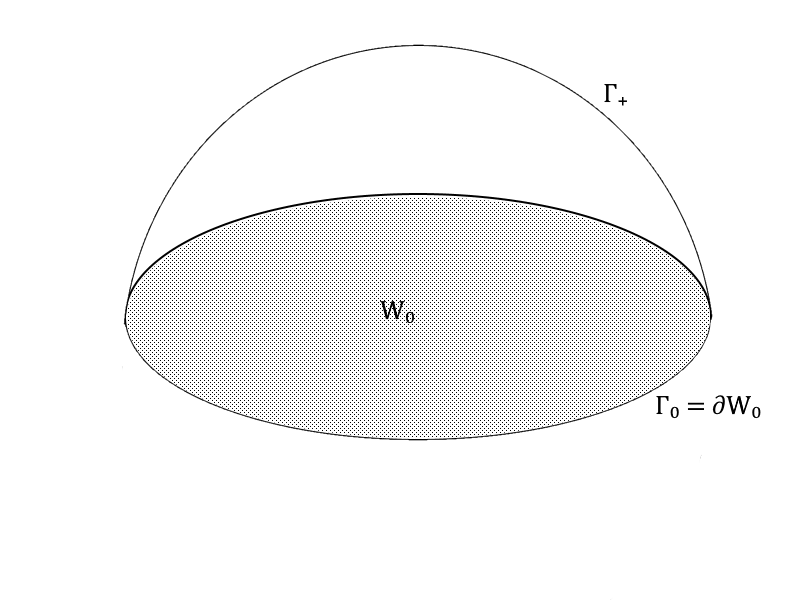
\includegraphics[width=\linewidth]{estimate homotopy.png}
\end{subfigure}
\caption{An illustration of the proof of Lemma \ref{mollifier sublemma}. On the left, the relative scales of balls involved in the proof of the lemma for $\gamma \ll 1$: $V$ is much smaller than $B_\varepsilon$, which in turn is tiny compared to $W$. On the right, $\Gamma_+$ and $W_0$ have the same homology class and the same boundary $\Gamma_0$, and $W_0$ is a slight deformation of a small ball in $\RR^{d - 1}$, so an integral $\int_{\Gamma_+} \omega$ can be approximated by the integral of $\star_{W_0} \omega$ over a small ball.}
\label{estimating figures}
\end{figure}

\begin{lemma}[control on $u_\varepsilon$]\label{main mollifier lemma}
Let $q < \min(1/8, 1/(4(d - 1)))$. There exists $c > 0$ such that for every $0 < \Delta \lesssim 1$ such that for every $0 < \gamma \lesssim 1$ and every indicator function $u$ of a set $U$ of least perimeter such that
\begin{equation}\label{hypothesis on main mollifier lemma}
\int_{B_\Delta} \star |\psi| \cdot |\dif u| - \dif u \wedge \psi \leq \gamma \Delta^{d - 1},
\end{equation}
if we let $\varepsilon = \gamma^4\Delta$, $\sigma = \gamma^{1/(2(d - 1))}\Delta$, and $\varphi = u_\varepsilon$, then on $B_{\Delta - 2\sigma} \cap \{c\gamma^2 < \varphi < 1 - c\gamma^2\}$,
\begin{equation}\label{claim on main mollifier lemma}
(1 - o(\gamma^q)) |\psi| \cdot |\dif \varphi| \leq \star(\dif \varphi \wedge \psi)
\end{equation}
and for every $y \in (c\gamma^2, 1 - c\gamma^2)$,
\begin{equation}\label{claim 2 on main mollifier lemma}
\text{the level set } \partial \{\varphi > y\} \cap B_{\Delta - 2\sigma} \text{ is a }C^1\text{ hypersurface}.
\end{equation}
\end{lemma}
\begin{proof}
Let $\delta = \gamma^d > 0$.
By running a greedy algorithm, we construct a cover $\mathcal V = \{V_n: 1 \leq n \leq N\}$ of $\partial^* U \cap B_{\varepsilon(1 - 2\delta)}$ by balls of radius $2\delta\varepsilon$, centered on points $Q_n \in \partial^* U \cap B_{\varepsilon(1 - \delta)}$, which is \dfn{efficient} in the sense that the dilates $V_n/2 := B(Q_n, \delta\varepsilon)$ are disjoint.
We set $V_0 := B_\varepsilon \setminus B_{\varepsilon(1 - 2\delta)}$.

To bring the $\psi$ inside the convolution we compute
\begin{align*}
(|\psi| \cdot |\dif u|)_\varepsilon
&= \int_{B_\varepsilon} |\psi|(x - y) |\dif u|(x - y) \chi_\varepsilon(y) \dif y \\
&= \int_{B_\varepsilon} |\psi|(x) |\dif u|(x - y) \chi_\varepsilon(y) \dif y + \int_{B_\varepsilon} ||\psi|(x - y) - |\psi|(x)| \cdot |\dif u|(x - y) \chi_\varepsilon(y) \dif y
\end{align*}
and observe that $||\psi|(x - y) - |\psi|(x)| \lesssim \dist(x, y) \lesssim \varepsilon \lesssim \gamma^4$.
Since $\dif u$ is supported in $\bigcup_n V_n$, it follows that
\begin{equation}\label{sum over cover}
|\psi| \cdot |\dif \varphi| - \star(\dif \varphi \wedge \psi)
\leq O(\gamma^4) |\dif \varphi| + \sum_{n=0}^N (1_{V_n}(|\psi| \cdot |\dif u| - \star(\dif u \wedge \psi)))_\varepsilon.
\end{equation}

We claim that there exists $c > 0$ such that on $B_\sigma \cap \{c\gamma^2 < \varphi < 1 - c\gamma^2\}$,
\begin{equation}\label{V0 case}
(1_{V_0}(|\psi| \cdot |\dif u| - \star(\dif u \wedge \psi)))_\varepsilon \lesssim \gamma |\dif u|_\varepsilon.
\end{equation}
The proof of (\ref{V0 case}) is essentially given by \cite[pg92]{Giusti77}, so we just sketch it.
For $y \in V_0$, $\chi_\varepsilon(x - y) \lesssim \delta/\varepsilon^d$, so using Proposition \ref{doubling dimension}, one can show
$$\int_{V_0} \chi_\varepsilon(x - y)(|\psi| \cdot |\dif u| - \star(\dif u \wedge \psi))(y) \dif y \lesssim \frac{\gamma^d}{\varepsilon}.$$
Here we used $||\psi||_{L^\infty} \lesssim 1$.
One can use \cite[Lemma 7.1]{Giusti77}, the assumption $c\gamma^2 < \varphi < 1 - c\gamma^2$, and the fact that $g$ is a perturbation of the euclidean metric to obtain
$$\int_{B_\varepsilon} \chi_\varepsilon(x - y) |\dif u|(y) \dif y \gtrsim \frac{\gamma^{d - 1}}{\varepsilon}$$
which then implies (\ref{V0 case}).

Since $\mathcal V$ is efficient, we can sum (\ref{V0 case}) and Lemma \ref{mollifier sublemma} over $n$ in (\ref{sum over cover}) to show that (\ref{claim on main mollifier lemma}) holds.
In particular near $\varphi^{-1}(y) \cap B_{\Delta - 2\sigma}$, where $y \in (c\gamma^2, 1 - c\gamma^2)$, one has $|\dif u| > 0$.
Therefore $u$ is a $C^1$ submersion by \cite[Lemma 7.1]{Giusti77}, thus (\ref{claim 2 on main mollifier lemma}) holds.
\end{proof}

\begin{lemma}
Suppose that $u = 1_U$ where $U$ has locally finite perimeter, $w = u_\varepsilon$, and $V = \{w > y\}$ where $y \in (0, 1)$.
Then for any submanifold $\iota: E \to M$ and $0 < \varepsilon \lesssim 1$,
\begin{equation}\label{Giusti125}
x|E \cap (U \Delta V)| \leq \frac{1}{\min(y, 1 - y)} \int_E |w - u| \iota^*(\star 1).
\end{equation}
Moreover, if $0 < \tau \lesssim 1$, then
\begin{align}
\int_{B_\tau} \star |w - u| &\lesssim \varepsilon |B_{\tau + \varepsilon} \cap \partial^* U|, \label{Giusti711}\\
\int_{B_\tau} \star (|\dif w| - |\dif u|) &\lesssim |(B_{\tau + \varepsilon} \setminus B_\tau) \cap \partial^* U|. \label{Giusti712}
\end{align}
\end{lemma}
\begin{proof}
The estimate (\ref{Giusti125}) is a straightforward modification of \cite[Lemma 1.25]{Giusti77}.
The estimates (\ref{Giusti711}, \ref{Giusti712}) follow from \cite[Lemma 7.2]{Giusti77} where we use the fact that for $\tau \lesssim 1$, we can impose normal coordinates and compare $\star 1$ to the euclidean volume form using (\ref{expand volume form}).
\end{proof}

We now state our main mollification result.
On first reading, it may help to take $P_n = P$, $(x^\mu_n) = (x^\mu)$, $\omega = \star \dif x^\mu$, and $\Delta_n = 1$.
The proof can be viewed as generalizing \cite[Lemma 7.5]{Giusti77}.

\begin{proposition}\label{mollifier quant}
Let $q < \min(1/8, 1/(4(d - 1)))$.
Let $(P_n)$ be a precompact sequence in $M$ and $0 < \Delta_n \lesssim 1$.
Let $U_n$ be a set of least perimeter in $B_n := B(P_n, \Delta_n)$, $(x^\mu_n)$ be a normal or stereographic coordinate system at $P_n$, let $\psi^n$ be given by (\ref{d1 form}), and
$$\gamma_n := \Delta_n^{1 - d} \int_{B_n} \star |\psi^n| \cdot |\dif 1_{U_n}| - \dif 1_{U_n} \wedge \psi^n.$$
If $(\gamma_n) \in \ell^1$ then for almost every $t \in (0, 1)$ and every $n \in \NN$ there exists a set $V_n$ with $C^1$ boundary in $tB_n := B(P_n, t\Delta_n)$ such that for $n \gg 1$,
\begin{align}
|\partial V_n \cap tB_n| &\leq \eta(V_n, t\Delta_n) + o(\gamma_n \Delta_n^{d - 1}), \label{mollifier quant1}\\
||\partial^* U_n \cap tB_n| - |\partial V_n \cap tB_n|| &\ll \gamma_n \Delta_n^{d - 1}, \label{mollifier quant2}
\end{align}
on $B(P_n, t(1 - 2\sigma_n)\Delta_n)$, where $\sigma_n := \gamma_n^{1/(2(d - 1))}$, one has
\begin{equation}
\star(\normal_{V_n} \wedge \psi^n) \geq |\psi^n| \cdot (1 - o(\gamma^q)), \label{mollifier quant4}
\end{equation}
and for almost every $s \in (0, t]$ and every $d-1$-form $\omega_n$ defined near $P_n$,
\begin{equation}\label{mollifier quant3}
\left|\int_{sB_n} \dif(1_{U_n} - 1_{V_n}) \wedge \omega_n\right| \ll \gamma_n \Delta_n^{d - 1} ||\omega_n||_{C^1}.
\end{equation}
\end{proposition}
\begin{proof}
In this proof, we shall assume that the constants furnished by the above results are uniform in $n$; this is possible by Remark \ref{independence of constants} and the compactness of $\overline{\{P_n: n \in \NN\}}$.

Draw $t$ uniformly at random, let $w_n := (u_n)_{\Delta_n \gamma_n^4}$, let $c, q$ be as in Lemma \ref{main mollifier lemma}, and let $a_n = c\gamma_n^2$, $b_n = 1 - c\gamma_n^2$.
By the coarea formula, Proposition \ref{Coarea2},
$$\int_{tB_n} \star |\dif w_n| = \int_0^1 |\partial^* \{w_n > y\} \cap tB_n| \dif y \geq \int_{a_n}^{b_n} |\partial^* \{w_n > y\} \cap tB_n| \dif y,$$
so by the mean value theorem, there exists $y_n \in (a_n, b_n)$ such that
$$|\partial^* \{w_n > y_n\} \cap tB_n| \leq \frac{1}{b_n - a_n} \int_{tB_n} \star |\dif w_n|.$$
We then set $V_n := \{w_n > y_n\}$, $v_n := 1_{V_n}$, so $V_n$ has $C^1$ boundary in $tB_n$ by (\ref{claim 2 on main mollifier lemma}), and by the above computation,
\begin{equation}\label{MVT mollifier}
|V_n \cap tB_n| \leq \frac{1}{1 - 2c\gamma_n^2} \int_{tB_n} \star |\dif w_n|.
\end{equation}
Since $\grad w_n$ is normal to the level sets of $w_n$, $\normal_{V_n} = \dif w_n/|\dif w_n|$.
Hence (\ref{mollifier quant4}) is a consequence of (\ref{claim on main mollifier lemma}).
The remaining estimates are consequences of the following claim:

\begin{claim}
Let $s \in (0, t]$ be chosen uniform at random and $\Gamma_n := \partial(sB_n)$.
Then almost surely, 
\begin{align}
||u_n - v_n||_{L^1(\Gamma_n)} &\ll \Delta_n^{d - 1} \gamma_n \label{trace of vn} \\
|\partial V_n \cap sB_n| &\leq |\partial^* U_n \cap sB_n| + o(\Delta_n^{d - 1} \gamma_n). \label{difference of surface area}
\end{align}
\end{claim}
\begin{proof}[Proof of claim]
By (\ref{Giusti711}) and Proposition \ref{doubling dimension},
$$\limsup_{n \to \infty} \Delta_n^{1 - d} \gamma_n^{-4} \int_{sB_n} \star |u_n - w_n| \lesssim \limsup_{n \to \infty} \Delta_n^{2-d} |\partial^* U_n \cap sB_n| \lesssim \sup_n \Delta_n \lesssim 1.$$
Differentiating in $s$, we see that
$$||u_n - w_n||_{L^1(\Gamma_n)} \ll \Delta_n^{d - 1} \gamma_n^3$$
almost surely. So by (\ref{Giusti125}),
$$||u_n - v_n||_{L^1(\Gamma_n)} \lesssim \gamma_n^{-2} ||u_n - w_n||_{L^1(\Gamma_n)} \ll \Delta_n^{d - 1} \gamma_n$$
almost surely, proving (\ref{trace of vn}).
Now let
$$f(r) = \sum_{n=1}^\infty \gamma_n \Delta_n^{1 - d} \int_{rB_n} \star |\dif u_n|.$$
Then $f' \geq 0$, and by Proposition \ref{doubling dimension}, $f(1) \lesssim \sum_n \gamma_n < \infty$.
So almost surely,
$$f(s + \gamma_n^4) - f(s) \lesssim \gamma_n^4$$
and hence
$$\int_{(s + \gamma_n^4)B_n \setminus sB_n} \star |\dif u_n| \lesssim \gamma_n^3 \Delta_n^{d - 1}.$$
From (\ref{Giusti712}) it follows that
$$\int_{sB_n} \star |\dif w_n| \leq \int_{sB_n} \star |\dif u_n| + o(\gamma_n^2).$$
By (\ref{MVT mollifier}) we conclude that (\ref{difference of surface area}) holds almost surely.
\end{proof}

For $s = t$, the estimate (\ref{mollifier quant2}) is the conjunction of (\ref{trace of vn}), (\ref{difference of surface area}), and (\ref{a priori estimate 1});
(\ref{mollifier quant1}) is the conjunction of (\ref{mollifier quant2}), (\ref{a priori estimate 1}), the fact that $U_n$ has least perimeter, and (\ref{trace of vn}).

It remains to establish (\ref{mollifier quant3}).
Integrating by parts,
$$\left|\int_{sB_n} \dif (u_n - v_n) \wedge \omega_n\right| \leq ||\omega_n||_{L^\infty} ||u_n - v_n||_{L^1(\Gamma_n)} + ||\dif \omega_n||_{L^\infty} \int_0^t ||u_n - v_n||_{L^1(\partial(sB_n))} \dif s.$$
By (\ref{trace of vn}),
$$\limsup_{n \to \infty} ||\omega_n||_{C^1}^{-1} \gamma_n^{-1} \Delta_n^{1 - d} \left|\int_{sB_n} \dif(u_n - v_n) \wedge \omega_n\right| \leq \limsup_{n \to \infty} \int_0^s \gamma_n^{-1} \Delta_n^{1 - d} ||u_n - v_n||_{L^1(\partial(rB_n))} \dif r.$$
Moreover, (\ref{trace of vn}) holds with $s$ replaced by almost any $r$, so
$$f_n(r) := \gamma_n^{-1} \Delta_n^{1 - d} ||u_n - v_n||_{L^1(\partial(rB_n))}$$
satisfies $(f_n) \in \ell^\infty([0, 1] \to L^\infty)$, and $f_n \to 0$ almost everywhere.
So by Fatou's lemma,
\begin{align*}
0 \leq \limsup_{n \to \infty} ||\omega_n||_{C^1}^{-1} \gamma_n^{-1} \Delta_n^{1 - d} \left|\int_{tB_n} \dif(u_n - v_n) \wedge \omega_n\right| &\leq \int_0^t \lim_{n \to \infty} f_n(r) \dif r = 0. \qedhere
\end{align*}
\end{proof}


%%%%%%%%%%%%%%%%%%%%%%%%%%%%%%%%%%%%%%%%%%%%%%
\section{Regularity of minimal hypersurfaces}\label{Plateau section}
\subsection{Approximate conormal one-form}
In this section we prove Theorem \ref{main lma}.
To set up the proof, recall that we can cover any manifold $M$ of constant sectional curvature $K \in \RR$ by charts $(x^\mu)$ in which the metric takes the form 
\begin{equation}\label{constant sectional curvature metric}
g_{\mu\nu} = \frac{\delta_{\mu\nu}}{(1 + K|x|^2/4)^2}.
\end{equation}
We fix such a chart and its origin $O$, where $x = 0$.
Consider a smooth family $(\Phi^P)_{P \in M}$ of oriented isometries $M \to M$, such that $\Phi^O = \id_M$ and $\Phi^P(P) = O$.
We write 
$$\partial^P_\mu := \Phi^P_* \partial_{x^\mu}.$$
Note that the choices of $(x^\mu)$ and $(\Phi^P)$ amount to selecting an oriented coordinate frame based at $P$ in which the metric takes the form (\ref{constant sectional curvature metric}).
The family of frames $(\partial^P_\mu)$ is uniquely determined up to a gauge transformation $\chi: M \to \SpOrth(TM)$, and so we will call a quantity \dfn{gauge-invariant} if it does not depend on the choice of $(x^\mu)$ or $(\Phi^P)$.

\begin{definition}
Let $U \subset M$ be a set of locally finite perimeter. Its \dfn{approximate conormal $1$-form} is defined for $P \in \partial U$,
$$\normal_U(P, r) := \frac{\int_{B(P, r)} \partial^P_\mu 1_U \star 1}{|\partial^* U \cap B(P, r)|} \dif x^\mu_P(P) \in T'_PM.$$
\end{definition}

\begin{lemma}
Let $U$ be a set of locally finite perimeter, then:
\begin{enumerate}
\item $\normal_U(P, r)$ is gauge-invariant.
\item For $r$ fixed, $\normal_U(P, r)$ is a continuous $1$-form along $\partial U$.
\item For $\star|\dif 1_U|$-almost every $P \in \partial U$,
\begin{equation}\label{convergence of conormal}
\lim_{r \to 0} \normal_U(P, r) = \normal_U(P).
\end{equation}
\item One has $|\normal_U(P, r)| \leq e^{C|K|r^2}$.
\end{enumerate}
\end{lemma}
\begin{proof}
For the gauge-invariance, let $\chi \in \SpOrth(T_PM)$ be a rotation.
Acting $\chi$ on $\normal_U(P, r)$ we obtain
$$\frac{\int_{B(P, r)} \chi^\nu_\mu \partial^P_\nu 1_U \star 1}{|\partial^* U \cap B(P, r)|} (\chi^{-1})_\lambda^\mu \dif x^\lambda_P(P) = \normal_U(P, r).$$ 
The continuity is clear, and (\ref{convergence of conormal}) follows from the Lebesgue differentiation theorem.
Finally we compute for $M := |\partial^* U \cap B(P, r)|$ that 
\begin{align*}
|\normal_U(P, r)|^2 &= g^{\mu\nu}_P(P) M^{-2} \left(\int_{B(P, r)} \partial^P_\mu 1_U \star 1\right) \left(\int_{B(P, r)} \partial^P_\nu 1_U \star 1\right) \\
&= \sum_\mu M^{-2} \left(\int_{B(P, r)} \partial^P_\mu 1_U \star 1\right)^2.
\end{align*}
Taking square roots and using the triangle inequality,
\begin{align*}
|\normal_U(P, r)| &\leq \frac{1}{M} \int_{B(P, r)} \sqrt{\sum_\mu |\partial^P_\mu 1_U|^2} \star 1 \leq \frac{1}{M} \max_\mu \int_{B(P, r)} |g^P_{\mu\mu}| \star |\dif 1_U| \\
&\leq \max_\mu ||g_{\mu\mu}||_{C^0(B(O, r))}.
\end{align*}
The claim now easily follows from the formula (\ref{constant sectional curvature metric}) for the metric.
\end{proof}

In order to use the previous lemma we need to show that approximate conormal $1$-form converges locally uniofrmly.
Therefore we need to control its oscillation.
This is accomplished by the de Giorgi lemma, and the main term in the de Giorgi lemma is called the excess.

\begin{definition}
The \dfn{excess} of a set $U \subset M$ of locally finite perimeter at $P \in \partial U$ and in the open set $A \ni P$ is 
$$\Exc_A(U, P) := |\partial^* U \cap A| - \sqrt{g^{\mu\nu}_P(P) \left(\int_A \partial^P_\mu 1_U \star 1\right) \left(\int_A \partial^P_\nu 1_U \star 1\right)}.$$
For $\rho > 0$ we write $\Exc_\rho(U, P) := \Exc_{B(P, \rho)}(U, P)$.
\end{definition}

\begin{lemma}
Let $U$ be a set of locally finite perimeter, let $A$ be an open set with Lipschitz boundary, and let $P \in A$.
Then $\Exc_A(U, P)$ is gauge-invariant and $g^{\mu\nu}_P(P) = \delta^{\mu\nu}$.
\end{lemma}
\begin{proof}
The gauge-invariance is analogous to the proof for $\normal_U(P, r)$, and the computation $g^{\mu\nu}_P(P) = \delta^{\mu\nu}$ follows because $g_{\mu\nu} = \delta_{\mu\nu}$.
\end{proof}

\begin{lemma}
Let $U$ be a set of locally finite perimeter, let $A$ be a Lipschitz open set such that
$$|\partial^* U \cap A| \leq C(\diam A)^{d - 1},$$
and let $P \in A$. Then:
\begin{enumerate}
\item For every $P' \in A$,
\begin{equation}\label{translation invariance}
|\Exc_A(U, P) - \Exc_A(U, P')| \leq C|K|(\diam A)^{d + 1}.
\end{equation}
\item If $P \in A' \subseteq A$, and $|\partial^* U \cap A| \geq C(\diam A)^{d - 1}$, then
\begin{equation}\label{approximate monotone}
-C |K| (\diam A)^{d + 1} \leq \Exc_{A'}(U, P) \leq \Exc_A(U, P) + C |K|(\diam A)^{d + 1}.
\end{equation}
\end{enumerate}
The hypotheses of this lemma are met if $A$ is a ball and $|\partial U \cap A| \leq 2\eta(U, A)$.
\end{lemma}
\begin{proof}
We first bound
\begin{align*}
|\Exc_A(U, P) - \Exc_A(U, P')| &= \left|\left|\int_A \partial^P_\mu 1_U \star 1 \dif x^\mu_P(P)\right| - \left|\int_A \partial^{P'}_\mu 1_U \star 1 \dif x^\mu_{P'}(P')\right|\right| \\
&\lesssim \max_\mu \int_A |\partial^P_\mu - \partial^{P'}_\mu| \star |\dif 1_U| \\
&\lesssim \max_\mu |\partial^P_\mu - \partial^{P'}_\mu| \cdot L(\diam A)^{d - 1}.
\end{align*}
To estimate this, we recall that since the excess is gauge-invariant, we may apply a gauge transformation $\chi$ to assume that $\Psi := \Phi^{P'} \circ (\Phi^P)^{-1}$ preserves the geodesic through $P, P'$.
Then by Lemma \ref{Coxeter estimate}, on $T_QM$, $Q \in A$,
\begin{align*}
|\partial^P_\mu - \partial^{P'}_\mu| &= |\Phi^P_* \partial_\mu - \Phi^{P'}_* \partial_\mu| \leq |\id - \Psi| \cdot |\partial_\mu|
\lesssim |K| \dist(Q, P) \dist(P', P) + |K| \dist(P', P)^2 \\
&\lesssim |K| (\diam A)^2.
\end{align*}

To deduce the positivity, we compute for $\rho := \diam A'$ that
\begin{align*}
\sqrt{g^{\mu\nu}_P(P) \left(\int_{A'} \partial^P_\mu 1_U \star 1\right) \left(\int_{A'} \partial^P_\nu 1_U \star 1\right)} &\leq \sqrt{\sum_\mu \left(\int_{A'} \partial_\mu^P 1_U \star 1\right)^2} \\
 & \leq \max_\mu ||\partial^P_\mu||_{C^0(A')} \cdot |\partial^* U \cap A'| \leq e^{CK\rho^2} |\partial^* U \cap A'| \\
 & \leq |\partial^* U \cap A'| + CK\rho^{d + 1}.
\end{align*}
The proof of monotonicity is similar.

Finally, if $A$ is a ball and $|\partial U \cap A| \leq 2\eta(U, A)$, then $\eta(U, A) \sim (\diam A)^{d - 1}$ by Proposition \ref{doubling dimension}.
To complete the proof we just note that $|\partial U \cap A| \geq \eta(U, A)$, so $|\partial U \cap A| \sim \eta(U, A) \sim (\diam A)^{d - 1}$.
\end{proof}

\begin{proposition}[de Giorgi lemma]\label{de Giorgi}
There exist $C > 0$, $c > 0$, and $\rho_* > 0$, such that for every $P \in M$, $\rho$ such that $0 < \rho < \rho_*$, and set $U \subset M$ of least perimeter such that 
$$\Exc_\rho(U, P) \leq c\rho^{d - 1},$$
we have 
$$\Exc_{\rho/2}(U, P) \leq 2^{-d} \Exc_\rho(U, P) + C|K|\rho^{d + 1}.$$
The constants $C, c, \rho_*$ only depend on $d$ for $|K| \lesssim 1$ (but may explode as $|K| \to \infty$).
\end{proposition}

\subsection{Reduction to the de Giorgi lemma}
We defer the proof of the de Giorgi lemma to \S\ref{proof of De Giorgi}.
Here we show that it implies Theorem \ref{main lma}.

\begin{lemma}
Assume the de Giorgi lemma.
Let $U$ be a set of least perimeter and $2 \leq d \leq 7$.
Then there is an open cover $\mathcal V$ of $\partial U$ by sets $V \in \mathcal V$, and constants $0 < \rho(V) < \rho_*$, so that for every $P \in V$,
$$\Exc_{\rho(V)}(U, P) \leq c\rho(V)^{d - 1}.$$
\end{lemma}
\begin{proof}
We first check that the desired inequality holds on the reduced boundary:

\begin{claim}
For each $P \in \partial^* U$ one has
$$\lim_{\rho \to 0} \rho^{1 - d} \Exc_\rho(U, P) = 0.$$
\end{claim}
\begin{proof}[Proof of claim]
Let $u = 1_U$, and recall the notation of Proposition \ref{blowup theorem}. If the lemma fails, then we can find $0 < \rho_n < 1/n$ and $\delta > 0$ such that 
$$\int_{B(P, \rho_n)} \star |\dif u| - \sqrt{\sum_{\mu = 0}^{d - 1} \left[\int_{B(P, \rho_n)} \star_{\partial U} \partial_\nu u\right]^2} > \delta \rho_n^{d - 1}.$$
At scale $\rho$, the difference between the pullback metric $\exp_P^* g$ and the euclidean metric on $T_PM$ is $O(K\rho^2)$, so if we denote by $v_n$ the tangent rescaling of $u$ to scale $\rho_n$, then for any sufficiently large $n$,
$$\int_{B'(0, 1)} \star |\dif v_n| - \left|\int_{B'(0, 1)} \dif v_n \star 1\right| \gtrsim \delta,$$
where $\int_{B'(0, 1)} \dif v_n \star 1$ needs to be understood as a vectorial integral.
By Proposition \ref{blowup theorem}, by taking subsequences we may assume that the tangent rescaling converges in the sense of the Miranda stability theorem to the indicator function $w$ of a half-space $C$ with $0 \in \partial C$.
But $B'(0, 1)$ is an open ball which contains the origin, so $\partial B'(0, 1)$ is transverse to $\partial C$.
Therefore, pursuant to Remark \ref{transversality},
\begin{equation}\label{c3 is zero}
\int_{B'(0, 1)} \star |\dif w| - \left|\int_{B'(0, 1)} \dif w \star 1\right| \gtrsim \delta,
\end{equation}
but $\partial C$ is a hyperplane, thus the left-hand side of (\ref{c3 is zero}) is $0$, which is a contradiction.
\end{proof}

Now let $Q \in \partial^* U$.
Then by the claim, there exists $\delta_* > 0$ such that for $0 < \delta < \delta_*$,
$$\Exc_\delta(U, Q) \leq \frac{c\delta^{d - 1}}{2^d}.$$
Then we can choose $\delta < \min(\delta_*, \rho_*)$ so small depending on $K$ that
$$\frac{c}{4^d} + C|K|\delta^2 \leq \frac{c}{2^d}.$$
Now if $P \in \partial U \cap B(Q, (2^{-1} - 2^{(d - 1)/d})\delta)$ and $\rho := 2^{(d - 1)/d}\delta$, then $B(P, \rho) \subseteq B(Q, \delta/2)$ and so by the de Giorgi lemma,
\begin{align*}
\Exc_\rho(U, P) &\leq \Exc_{\delta/2}(U, Q) + C|K|\delta^{d + 1} \leq \frac{\Exc_\delta(U, Q)}{2^d} + C|K|\delta^{d + 1} \\
&\leq \left(\frac{c}{4^d} + C|K|\delta^2\right)\delta^{d - 1} \leq \frac{c\delta^{d - 1}}{2^d} \leq \rho^d.
\end{align*}
Since $\partial^* U$ is dense in $\partial U$, we can define our open cover to consist of balls $V := B(Q, (2^{-1} - 2^{(d - 1)/d})\delta)$ for $Q \in \partial^* U$ and $\delta = \delta(Q)$ as above, and let $\rho(V) := 2^{(d - 1)/d}\delta$.
\end{proof}


\begin{proposition}\label{implication of DGL}
    Assume the de Giorgi lemma. Let $U$ be a set of least perimeter.
    If $2 \leq d \leq 7$ then for $P \in V$, $V \in \mathcal V$, and for every $0 < s < r < \rho(V)$,
    \begin{equation}\label{LC Cauchy}
    %|\normal_U(P, r) - \normal_U(P, s)| \lesssim \sqrt{\left(1 - |K| \log \frac{r}{\rho(V)}\right)\frac{r}{\rho(V)}}.
    |\normal_U(P, r) - \normal_U(P, s)| \lesssim \sqrt{\frac{r \Japan K}{\rho(V)}}.
    \end{equation}
\end{proposition}
\begin{proof}
To fix notation, let
$\xi := \normal_{U, r}(P)$, $\eta = \normal_{U, s}(P)$, $m := |\partial^* U \cap B(P, s)|$, $M := |\partial^* U \cap B(P, r)|$, $\rho := \rho(V)$, and $\gamma_n := \Exc_{\rho/2^n}(U, P)$.

\begin{claim}
The proposition holds if $r/2 < s < r := \rho/2^n$.
% $$|\xi - \eta| \lesssim \sqrt{\left[\frac{1}{\rho} + |K|\log_2\left(\frac{\rho}{r}\right)\right] r}.$$
\end{claim}
\begin{proof}[Proof of claim]
We first estimate
$$|\xi - \eta|^2 = |\xi|^2 + |\eta|^2 - 2 g^{-1}(\xi, \eta) \leq 2(1 - g^{-1}(\xi, \eta)) + C|K|r^2.$$
To estimate the right-hand side we write 
$$m(1 - g^{-1}(\xi, \eta)) = \int_{B(P, s)} \star(|\dif 1_U| - g^{-1}(\xi, \dif x^\mu_P(P)) \partial^P_\mu 1_U).$$
Now we bound 
$$ g^{-1}(\xi, \dif x^\mu_P(P)) \partial^P_\mu 1_U \leq |\xi| \cdot |\dif 1_U| \cdot \max_\mu |\partial^P_\mu| \leq e^{C|K|r^2} |\dif 1_U|,$$
which implies that, since $s \leq r$,
$$\int_{B(P, s)} \star(|\dif 1_U| - g^{-1}(\xi, \dif x^\mu_P(P)) \partial^P_\mu 1_U) \leq \int_{B(P, r)} \star(e^{C|K|r^2} |\dif 1_U| - g^{-1}(\xi, \dif x^\mu_P(P)) \partial^P_\mu 1_U).$$
By Proposition \ref{doubling dimension}, the first term integrates to $\leq M + C|K|r^{d + 1}$, and so by definition of $\xi$,
\begin{align*}
\int_{B(P, r)} \star(e^{CKr^2} |\dif 1_U| - g^{-1}(\xi, \dif x^\mu_P(P)) \partial^P_\mu 1_U) &\leq M(1 - |\xi|^2) + C|K|r^{d + 1}\\
&\leq 2M(1 - |\xi|) + C|K|r^{d + 1}.
\end{align*}
But $M(1 - |\xi|)$ is exactly the definition of $\Exc_r(U, P)$, so putting everything together and using Proposition \ref{doubling dimension} to bound $m \gtrsim s^{d - 1} \gtrsim r^{d - 1}$, we have the bound 
\begin{equation}\label{just need the excess}
|\xi - \eta|^2 \lesssim r^{1 - d} \Exc_r(U, P) + |K|r^2.
\end{equation}
Then, since $r = \rho(V)/2^n$, $\Exc_r(U, P) = \gamma_n$, and for $C' := C|K|\rho^{d + 1}$ we have the recurrence relation 
$$\gamma_{k + 1} \leq \frac{\gamma_k}{2^d} + \frac{C'}{2^{k{d + 1}}},$$
by the de Giorgi lemma.
By induction, then,
$$\gamma_n \leq \frac{\gamma_0}{2^{nd}} + C' \sum_{k=0}^n \frac{1}{2^{k(d + 1)} 2^{(n - k)d}}.$$
We compute this sum as 
$$\sum_{k=0}^n \frac{1}{2^{k(d + 1)} 2^{(n - k)d}} = \frac{2^{n + 1} - 1}{2^{n(d + 1)}} \leq \frac{2^{n + 1}}{2^{n(d + 1)}} = \frac{2}{2^{nd}}.$$
In summary, 
$$\gamma_n \leq \frac{\gamma_0 + 2C'}{2^{nd}} \leq \frac{c\rho^{d - 1} + 2C'}{2^{nd}}.$$
% $$\gamma_n \leq \frac{\gamma_0}{2^{nd}} + \frac{nC'}{2^{nd}} \leq \left[\frac{1}{\rho} + C|K|\log_2\left(\frac{\rho}{r}\right)\right] r^d.$$
% |\xi - \eta|^2 &\lesssim \left[\frac{1}{\rho} + |K|\log_2\left(\frac{\rho}{r}\right) + |K|r\right] r.
The result now follows from (\ref{just need the excess}).
\end{proof}

In general we can find $n, m \in \NN$ such that $\rho/2^{n + 1} < \xi \leq \rho/2^n$ and $\rho/2^{n + m + 1} < \eta \leq \rho/2^{n + m}$.
Writing $\zeta_\ell := \normal_{U, \rho/2^\ell}$ we have by the claim that
% \begin{align*}
% |\xi - \eta| &\leq |\xi - \zeta_n| + \sum_{\ell=n}^{n + m - 1} |\zeta_\ell - \zeta_{\ell + 1}| + |\zeta_{n + m} - \eta| \\
% &\lesssim \rho^{-1/2} \left[\sqrt{\frac{1 + |K|n}{2^{nd}}} + \sum_{\ell=n}^{n + m - 1} \sqrt{\frac{1 + |K|\ell}{2^{\ell d}}} + \sqrt{\frac{1 + |K|(n + m)}{2^{(n + m)d}}}\right] \\
% &\lesssim \sqrt{\frac{1}{2^{nd} \rho}} \left[\sqrt{1 + |K|n} + \sum_{\ell=0}^\infty 2^{-\ell d} + |K|^{1/2} \sum_{\ell=0}^\infty 2^{-\ell(d - 1)}\right] \\
% &\lesssim \sqrt{\frac{1 + |K|n}{2^{nd} \rho}}. \qedhere
% \end{align*}
\begin{align*}
|\xi - \eta| &\lesssim |\xi - \zeta_n| + \sum_{\ell=n}^{n + m - 1} |\zeta_\ell - \zeta_{\ell + 1}| + |\zeta_{n + m} - \eta| \\
&\lesssim \sqrt{\frac{\Japan K}{\rho}} \left[2^{-nd/2} + \sum_{\ell=n}^{n + m - 1} 2^{-\ell d/2} + 2^{-(n + m) d/2} \right]\\
&\lesssim \sqrt{\frac{\Japan{K}}{2^{nd} \rho}} \left[1 + \sum_{\ell=0}^\infty 2^{-\ell d}\right] \lesssim \sqrt{\frac{\Japan{K}}{2^{nd} \rho}}. \qedhere
\end{align*}
\end{proof}

\begin{proof}[Proof of Theorem \ref{main lma} assuming the de Giorgi lemma]
By an elliptic bootstrapping argument it suffices to show that $\partial U$ is $C^1$.
Then, by Proposition \ref{locality of Caccioppoli}, it suffices to show that $\normal_U$ extends to a continuous $1$-form along $\partial U$.
But this is clear, because the continuous $1$-form $\normal_U(\cdot, r)$ approximates it locally uniformly by Proposition \ref{implication of DGL}.
\end{proof}

%%%%%%%%%%%%%%%%%%%%%%%%%%%%%%%%%

% \subsection{Remarks on the de Giorgi lemma}

% \subsubsection{Sketch of the proof}


% \subsubsection{The logarithmic loss}

% We cope with this by making some unnatural choices, which are the source of lack of translation-invariance. As such, compared to \cite{Miranda66, deGiorgi61} we have to pay with a logarithmic loss $-|K|\log \rho$.
% That the loss is logarithmic is a manifestation of the fact that in order to estimate the excess at scale $\rho \sim 2^{-n}$, we must invoke the approximate translation-invariance a total of $O(n)$ times, since the de Giorgi lemma is designed to allow induction on dyadic scales and we invoke the approximate translation-invariance $O(1)$ times at each inductive step.

%%%%%%%%%%%%%%%%%%%%%%%%%%%%%%%%%%%%%%%%%%
\section{Proof of the de Giorgi lemma}\label{proof of De Giorgi}
Since the proof of the de Giorgi lemma is long, we begin with a sketch.
Let $U$ be a set of least perimeter such that $O \in \partial U$, let $\psi$ be the vertical form, and fix a scale $\rho > 0$.
Since the excess is rotation-invariant, we may assume that $\partial U$ is almost horizontal in the sense that on average, $\normal_U \wedge \psi$ is approximately the volume form of $M$.
So by Proposition \ref{mollifier quant}, we may replace $\partial U$ with a $C^1$ submanifold $N$ of $M$ which is approximately minimal, and such that $O$ is close to $N$ and $N$ is almost horizontal in a pointwise sense; this is Lemma \ref{single mollify}.
Now we can invoke approximate translation-invariance of the excess to assume that in fact, $O \in N$, at the price of a loss of size $C|K|\rho^{d + 1}$.

Since we have an explicit choice of coordinates on $M$ and $N$ is approximately horizontal, we can find a function $w$ on an open subset of $\RR^{d - 1}$ whose graph is $N$; this is Lemma \ref{rep as a good graph}.
Moreover, the fact that $N$ is approximately minimal means that $w$ is an approximate solution of a certain quasilinear elliptic PDE.
Such an equation is close to the Plateau equation for $|x|^2 + |w(x)|^2$ small and so we can apply de Giorgi's estimates on the Plateau equation (Lemma \ref{Miranda42 quant}) to obtain a de Giorgi-type lemma for $w$, namely Lemma \ref{Miranda43}.
Here we have $|w(x)| \lesssim |x|$ since $O \in N$ and hence $w(0) = 0$.
Backtracking, we obtain analogous de Giorgi-type lemmata for $N$ (Lemma \ref{Miranda44}) and ultimately $U$, proving Proposition \ref{de Giorgi}.

\begin{remark}
The reason why Miranda's argument cannot be generalized verbatim is that it relies on an elementary estimate \cite[Lemma 4.1]{Miranda66} due to de Giorgi \cite{deGiorgi61} for the euclidean Laplace equation.
This is problematic for two reasons:

\begin{enumerate}
\item The proof of \cite[Lemma 4.1]{Miranda66} relies on the decomposition of harmonic functions on $\RR^{d - 1}$ into orthogonal harmonic polynomials, and an analogous result does not seem to be available for more general elliptic operators.
\item To apply \cite[Lemma 4.1]{Miranda66} (or more precisely, its consequence, Lemma \ref{Miranda42 quant}), we need to realize a function as a graph. This is unnatural on manifolds such as $\Sph^d$ and $\Hyp^d$ which do not have a natural product structure.
\end{enumerate}

One may be able to avoid these issues, and give a more natural proof of Theorem \ref{main lma}, via the phase transition theory, c.f. \S\ref{open problems}.
\end{remark}

\subsection{Minimal graphs case}
We turn to the details.
First we show that the de Giorgi lemma holds for $C^1$ hypersurfaces which are approximated by minimal graphs; this is an analogue of \cite[Teorema 4.3]{Miranda66}.

Recall that for a coordinate system $(x^\mu)$, we sometimes write $y := 0$, in which case we sum indices as $i, j, k = 1, \dots, d - 1$ and $\mu, \nu, \lambda = 0, \dots, d - 1$, and write $x := (x^i)$.
Here the coordinate system is centered on $O$, and chosen so the metric takes the form (\ref{constant sectional curvature metric}).

\begin{definition}
For $\Omega \subset \RR^{d - 1}$ open, define the smooth family of volume forms on $\Omega$,
$$\Lagrange(y, \xi) := \frac{\Japan{\xi}}{(1 + K(|x|^2 + y^2)/4)^{d - 1}} \dif x.$$
For each $w \in H^1(\Omega)$, the \dfn{Plateau energy} of $w$ is $\Lagrange(w, \dif w)$.
\end{definition}

\begin{lemma}\label{Plateau setup lemma}
Let $w \in C^1(\Omega)$, $\Omega \subseteq \RR^{d - 1}$, and let $\Psi_w(x) := (x, w(x))$. Let $N_w$ be the image of $\Psi_w$. Then:
\begin{enumerate}
\item The restriction of $g$ to $N_w$ pulls back as
\begin{equation}\label{restricted metric in isothermal coords}
\Psi_w^*(g|N_w)_{ij} = \frac{\delta_{ij} + \partial_i w \partial_j w}{(1 + K(|x|^2 + w^2)/4)^2}
\end{equation}
\item The induced volume form on $N_w$ pulls back as
\begin{equation}\label{restricted measure in isothermal coords}
\Psi_w^*(\iota_{\normal_{N_w}}(\star 1)) = \Lagrange(w, \dif w).
\end{equation}
\item The upwards conormal $1$-form is
\begin{equation}\label{conormal in isothermal coords}
\normal_U(x, w(x)) = \frac{\dif y - \partial_i w \dif x^i}{\Japan{\dif w}(1 + K(|x|^2 + w^2)/4)}.
\end{equation}
\end{enumerate}
\end{lemma}
\begin{proof}
We have $\Psi_w^0 = w$, $\Psi_w^i = x^i$, thus
\begin{align*}
\Psi_w^*(g|N_w)_{ij} &= g_{\mu\nu} \partial_i \Psi_w^\mu \partial_j \Psi_w^\nu \\
&= \frac{\delta_{\mu\nu}}{(1 + K(|x|^2 + w^2)/4)^2} (\partial_i \Psi_w^\mu \partial_j \Psi_w^\nu) \\
&= \frac{\delta_{ij} + \partial_i w \partial_j w}{(1 + K(|x|^2 + w^2)/4)^2},
\end{align*}
proving (\ref{restricted metric in isothermal coords}).
By \cite[(24)]{Petersen2008} we have $\det((\delta_{ij} + \partial_i w \partial_j w)_{ij}) = 1 + |\dif w|^2$, which gives (\ref{restricted measure in isothermal coords}).
Finally, it is well-known that (\ref{conormal in isothermal coords}) holds if $K = 0$, and otherwise we have a conformal map $\Phi: M \to \RR^d$ simply by forgetting the metric.
Then up to a scaling factor to account for length, $\Phi$ must preserve $\normal_U$.
Since the length of $(\dif y - \partial_i w \dif x^i)/\Japan{\dif w}$ is $1 + K(|x|^2 + w^2)/4$, (\ref{conormal in isothermal coords}) holds.
\end{proof}

% \begin{proposition}\label{Plateau wellposedness}
% On balls $B_\rho \subset \RR^{d - 1}$, $\rho \leq |K|^{-1/2}$, we can uniquely solve the Dirichlet problem for the Plateau equation for data which is small enough in $C^0(\partial B_\rho)$ depending on $K, d$.
% Moreover, every minimizer $w \in H^1(B_\rho)$ of the Plateau energy with $||w||_{L^\infty} \leq |K|^{-1/2}$ is an analytic solution of the Plateau equation on $B_\rho$, and its graph is a minimal hypersurface in $\Omega \times [-|K|^{-1/2}, |K|^{-1/2}] \subset M$.
% \end{proposition}
% \begin{proof}
% This is standard and we omit the details, but refer to \cite[Chapters 12-14]{Giusti77} for a discussion of the euclidean case.
% Taking a variation $w_t := w + tv$ of $\Lagrange(w, \dif w)$, where $v \in C^\infty_\cpt(B_\rho)$ and $\Lagrange$ is stationary at $w$,
% \begin{align*}
% 0 &= \frac{\dif}{\dif t} \int_{B_\rho} \Lagrange(w_t)
% = \int_{B_\rho} \partial_t \left[\frac{\Japan{\dif w_t}}{(1 + K(|x|^2 + w_t^2)/4)^{d - 1}}\right] \dif x \\
% &= \int_{B_\rho} \frac{\dif w_t \cdot \dif v}{(1 + K(|x|^2 + w_t^2))^{d - 1}} \dif x - (d - 1) \int_{B_\rho} \Japan{\dif w_t} \frac{2w_tKv/4}{(1 + K(|x|^2 + w_t^2)/4)^d} \dif x.
% \end{align*}
% Taking $t \to 0$ and integrating by parts we obtain the weak form of
% \begin{equation}\label{Plateau eqn}
% \dif^* \left[\frac{1}{(1 + K(|x|^2 + w^2)/4)^{d - 1}} \cdot \frac{\dif w}{\Japan{\dif w}}\right] + \frac{K(d - 1)}{2(1 + K(|x|^2 + w^2)/4)^d} \Japan{\dif w} = 0.
% \end{equation}
% This equation is second-order quasilinear so in the limit $||w||_{C^1} \to 0$, (\ref{Plateau eqn}) becomes the linear PDE
% \begin{equation}\label{linear Plateau eqn}
% Lw := -\dif^* \left[\frac{\dif w}{(1 + K|x|^2/4)^{d - 1}}\right] = h,
% \end{equation}
% where $h(x) := K(d - 1)/2 \cdot (1 + K|x|^2/4)^{-d}$ is analytic and $\gtrsim -|K|d$ on $B_\rho$ since $|x| \leq |K|^{-1/2}$ on $B_\rho$, and $L$ is uniformly elliptic of second order and analytic coefficients.
% We can decompose any $w$ solving (\ref{linear Plateau eqn}) as $w = u + v$ where $Lu = h$ and $u$ is trace-free, and $Lv = 0$ and $v|\partial B_\rho = w|\partial B_\rho$.
% By the maximum principle, $||v||_{C^0} = ||w||_{C^0(\partial B_\rho)}$ while $||u||_{C^0} \lesssim_{d, K} ||h||_{C^0} $

% This implies the uniqueness and the fact that candidate extensions $\tilde f$ of the Dirichlet data $f$ must satisfy $||\tilde f||_{C^0} \leq |K|^{-1/2}$.
% Now if $\max(\rho, ||w||_{L^\infty}) \leq |K|^{-1/2}$, then for $r \geq 0$, $(1 + K(|x|^2 + w^2)/4))^{-r} \leq 2^r$ is analytic on $\overline{B_\rho}$, so the analyticity follows by elliptic bootstrapping.
% An application of the direct method of the calculus of variations, using the regularity and the estimate $||\tilde f||_{C^0} \leq |K|^{-1/2}$, gives the existence.
% Finally, the minimality of the graph follows from (\ref{restricted measure in isothermal coords}).
% \end{proof}

In the sequel, all implied constants, and any constant called $C$, must only depend on $d$ for $K$ bounded.
They must also be independent of any function or set of least perimeter in consideration.
However, they may blow up as $K \to \infty$.

We fix $c_0 = c_0(d) \in (0, 1)$ to be chosen later, but small enough to meet the hypotheses of Lemma \ref{Miranda42 quant}.
We then let $c_1 = c_1(c_0, d) \in (0, c_0)$ be at most the constant obtained from Lemma \ref{Miranda42 quant}.

% \begin{lemma}\label{dGL same trace}
% Let $u, w \in C^1(B_\rho)$, $B_\rho \subset \RR^{d - 1}$, $\rho \leq 1$, be such that $w(0) = 0$ and 
% \begin{equation}\label{dGL same traces hyp}
% u|\partial B_\rho = w|\partial B_\rho, ~ ||u||_{C^1} \lesssim ||w||_{C^1} \leq c_1.
% \end{equation}
% Then
% \begin{equation}\label{dGL same traces concl}
% \int_{B_\rho} \Japan{\dif w} - \Japan{\dif u} \dif x = \int_{B_\rho} \Lagrange(w, \dif w) - \Lagrange(u, \dif u) + O(\rho^{d + 1})
% \end{equation}
% and similarly
% \begin{equation}\label{dGL same traces concl 2}
% \int_{B_\rho} \Japan{\dif w} - \Japan{\avg_\rho \dif w} \dif x = \int_{B_\rho} \Lagrange(w, \dif w) - \Lagrange(w, \avg_\rho \dif w) + O(\rho^{d + 1}).
% \end{equation}
% \end{lemma}
% \begin{proof}
% We prove (\ref{dGL same traces concl}) as the proof of (\ref{dGL same traces concl 2}) is similar.
% Let $F_w(x) = (1 + K(|x|^2 + w(x)^2)/4)^{1 - d}$ and similarly for $F_u$.
% We write out 
% \begin{equation}\label{dGL same traces proof}
% \int_{B_\rho} \Lagrange(w, \dif w) - \Lagrange(u, \dif u) = \int_{B_\rho} F_w(x) (\Japan{\dif w(x)} - \Japan{\dif u(x)}) + (F_w(x) - F_u(x)) \Japan{\dif u(x)} \dif x.
% \end{equation}
% Let $I := B_\rho \times (-M\rho, M\rho)$ where by (\ref{dGL same traces hyp}),
% $$M := \rho^{-1} \max(||w||_{C^0(B_\rho)}, ||u||_{C^0(B_\rho)}) \lesssim 1.$$
% Thus $\diam I \lesssim \rho$.
% In particular, we can dispose of the first term in (\ref{dGL same traces proof}) using $F_w(x) = 1 + O(|x|^2) + O(||w||_{C^0}^2)$, where of course $\max(|x|, |w(x)|) \leq \rho$.
% In order to bound $|F(x, w(x)) - F(w, u(x))|$ we estimate using (\ref{dGL same traces hyp}) that $||w - u||_{C^0} \lesssim \rho$.
% Now fix $x \in \RR^{d - 1}$ and observe that $D := \dist((x, w(x)), (x, u(x))) \leq \diam I \lesssim \rho$, thus
% \begin{align*}
% ||F_w - F_u||_{C^0} &\leq D(||\dif F_w||_{C^0} + ||\dif F_u||_{C^0}) \lesssim \rho^2. \qedhere
% \end{align*}
% \end{proof}

\begin{lemma}
Let $\beta, \rho > 0$, $w \in C^1(B_\rho)$, $w(0) = 0$, and $||\dif w||_{C^0} \leq c_1$. Then
\begin{equation}\label{compare Lagrangians}
\left|\int_{B_\rho} \Lagrange(w, \dif w) - \Lagrange(w, \avg_\rho \dif w) - \Japan{\dif w} \dif x + \Japan{\avg_\rho \dif w} \dif x\right|
\lesssim |K| \rho^{d + 1}.
\end{equation}
\end{lemma}
\begin{proof}
The left-hand side of (\ref{compare Lagrangians}) is
\begin{align*}
&\left|\int_{B_\rho} ((1 + K(|x|^2 + w(x)^2)/4)^{1 - d} - 1)(\Japan{\dif w} - \Japan{\avg_\rho \dif w}) \dif x\right| \\
&\qquad \lesssim_d |K| \int_{B_\rho} (|x|^2 + w(x)^2) \cdot \left|\Japan{\dif w} - \Japan{\avg_\rho \dif w}\right| \dif x.
\end{align*}
But $|B_\rho| \sim \rho^{d - 1}$, $|\Japan{\dif w} - \Japan{\avg_\rho \dif w}| \lesssim \exp(||\dif w||_{C^0}) \leq e^{c_1}$,
$$(|x|^2 + w(x)^2) \leq (1 + ||\dif w||_{C^0}^2) \rho^2 \lesssim e^{2c_1} \rho^2,$$
and since $c_1 \leq 1$ this gives the result.
\end{proof}

\begin{lemma}[de Giorgi lemma, minimal graphs]\label{Miranda43}
Let $\beta, \rho > 0$, $w \in C^1(B_\rho)$, and let $I_w$ be the cylinder in $M$, $I := \{|x| < \rho\}$.
If $w(0) = 0$ and $||\dif w||_{C^0} \leq c_1$,
\begin{align}
\int_{B_\rho} \Lagrange(w, \dif w) - \Lagrange(w, \avg_\rho \dif w) &\leq \beta \label{Miranda43 oscillation}, \\
\int_{B_\rho} \Lagrange(w, \dif w) &\leq \eta(N_w, I) + c_1 \beta \label{Miranda43 minimality},
\end{align}
then for any $0 < \alpha < 1$,
\begin{equation}\label{Miranda43 concl}
\int_{B_{\alpha \rho}} \Lagrange(w, \dif w) - \Lagrange(w, \avg_{\alpha \rho} \dif w) \leq (\alpha^{d + 1} + c_0) \beta + C|K|\rho^{d + 1}.
\end{equation}
\end{lemma}
\begin{proof}
Let $u$ be the harmonic function on $B_\rho$ which equals $w$ on $\partial B_\rho$.
By elliptic regularity, the maximum principle for harmonic functions, and (\ref{Miranda43 minimality}),
$$||u||_{C^1} \lesssim ||u||_{C^0} \leq ||w||_{C^0} \leq ||\dif w||_{C^1} \leq c_1.$$
In particular, $\Japan{\dif u} \lesssim 1$ and $u(x)^2 \lesssim |x|^2$, so
\begin{align*}
&\left|\int_{B_\rho} \Lagrange(w, \dif w) - \Lagrange(u, \dif u) - \Japan{\dif w} \dif x + \Japan{\dif u} \dif x\right| \\
&\qquad \leq |K| \int_{B_\rho} (|x|^2 + w(x)^2) \Japan{\dif w} \dif x + (|x|^2 + u(x)^2) \Japan{\dif u} \dif x 
\lesssim_d |K| \rho^{d + 1}.
\end{align*}
Since $u$ and $w$ have the same trace, $|N_u \cap I| \leq \eta(N_w, I)$, thus by (\ref{restricted measure in isothermal coords}),
\begin{align*}
\int_{B_\rho} \Lagrange(w, \dif w) - \Lagrange(u, \dif u) &\leq \int_{B_\rho} \Lagrange(w, \dif w) - \eta(N_w, I) \leq c_1 \beta.
\end{align*}
Moreover, we meet the hypotheses of (\ref{compare Lagrangians}).
So $w, u$ meet the hypotheses of Lemma \ref{Miranda42 quant} for some $\beta' \in [\beta, \beta + C|K|\rho^{d + 1}]$. 
We conclude from that lemma that (\ref{Miranda43 concl}) holds.
\end{proof}

% TODO: Move all this stuff into the previous section

% In order to estimate the excess $\Exc_{P, A} U$, we first observe that by Proposition \ref{doubling dimension} we have for $U$ satisfying $|\partial^* U \cap A| \lesssim \eta(U, A)$,
% \begin{equation}\label{noneccentric dimension}
% \sup_{P \in \partial^* U} \sup_{B(P, \rho) \subseteq A} \rho^{d - 1} \lesssim |\partial^* U \cap A| \lesssim (\diam A)^{d - 1}.
% \end{equation}

% \begin{lemma}[rotation invariance]\label{rotation invariance 2}
% The excess $\Exc_{P, A} U$ is well-defined: it does not depend on a choice of stereographic coordinates.
% \end{lemma}
% \begin{proof}
% Let $(\partial_\mu)$ and $(\partial_\mu')$ be two coordinate frames induced by two choices of stereographic coordinates based at $P$.
% From Remark \ref{rotation invariance} we see that there is an orthogonal matrix $O$ such that $\partial_\mu' = O_\mu^\nu \partial_\nu$, and then 
% \begin{align*}
% \sum_{\mu = 0}^{d - 1} \left[\int_A \star \partial_\mu' 1_U\right]^2 &= \sum_{\mu=0}^{d - 1} (O_\mu^\nu)^2 \left[\int_A \star \partial_\nu 1_U\right]^2 = \sum_{\mu = 0}^{d - 1} \left[\int_A \star \partial_\mu 1_U\right]^2. \qedhere 
% \end{align*}
% \end{proof}

% \begin{definition}
% Fix a choice of stereographic coordinates based at $P$, let $\psi$ be their associated vertical $d-1$-form, and let $A \ni P$.
% A set $U$ of locally finite perimeter is \dfn{horizontal on average} in $A$ if
% \begin{equation}\label{horizontal on average}
% \Exc_{P, A} U = \int_A \star |\dif 1_U| \cdot |\psi| - \dif 1_U \wedge \psi.
% \end{equation}
% \end{definition}

% Applying Lemma \ref{rotation invariance 2}, it follows that for $\rho$ small and $P, Q \in M$, we may always choose stereographic coordinates based at $P \in B(Q, \rho)$ so that a given set is vertical in $B(Q, \rho)$.\footnote{There are other notions of excess in the literature, such as the Allard excess \cite{Allard72,colding2011course}. The Allard excess $\Exc^{\mathrm{All}}_A U$ is diffeomorphism-invariant, but we found the de Giorgi excess more convenient to work with. However, one can show that if $U$ is horizontal on average and $P = Q$, then $\Exc^{\mathrm{All}}_A U$ is essentially the right-hand side of (\ref{horizontal on average}), so the distinction between $\Exc^{\mathrm{All}}_A U$ and $\Exc_{P, A} U$ turns out to be irrelevant.}

% \begin{lemma}[approximate translation invariance]
% Let $A \subset M$ be open and $P, Q \in A$, then
% \begin{equation}\label{translation invariance}
% \Exc_{P, A} U = \Exc_{Q, A} U + O((\diam A)^d).
% \end{equation}
% \end{lemma}
% \begin{proof}
% Let $\rho := \diam A$.
% We can choose stereographic coordinates based at $Q$, with vertical form $\psi_Q$, such that $U$ is horizontal on average.
% We then choose compatible stereographic coordinates based at $P$, thus $|\psi_P - \psi_Q| \lesssim \rho$ by (\ref{compatible verticals}).
% Integrating and using (\ref{noneccentric dimension}), we obtain 
% $$\int_A |\dif 1_U| \cdot |\psi_P| - \dif 1_U \wedge \psi_P \leq \int_A |\dif 1_U| \cdot |\psi_Q| - \dif 1_U \wedge \psi_Q + C\rho^d.$$
% Now $U$ may not be horizontal on average with respect to $\psi_P$. However, Taylor expanding the metric,
% $$\int_A \dif 1_U \wedge \psi_P \leq \sqrt{\sum_{\mu = 0}^{d - 1} \left[\int_A \star \partial^P_\mu 1_U\right]^2} + C\rho^d,$$
% which implies that
% $$\Exc_{P, A} U \leq \int_A |\dif 1_U| \cdot |\psi_P| - \dif 1_U \wedge \psi_P + C\rho^d$$
% and hence implies (\ref{translation invariance}).
% \end{proof}

% Applying (\ref{expand metric}) and (\ref{noneccentric dimension}), we obtain for open sets $A \subseteq A'$ that the excess is approximately monotone and nonnegative:
% \begin{align}
% -C \sup_{P \in \partial^* U} \sup_{B(P, \rho) \subseteq A} \rho^{d + 1} \leq \Exc_{P, A} U &\leq \Exc_{P, A'} U + C((\diam A')^{d + 1}). \label{approximate monotone}
% \end{align}
% In the case of balls we can refine the estimate (\ref{approximate monotone}):

% \begin{lemma}[monotonicity formula for excess]\label{monotonicity formula for excess}
% Let $U$ be a set of least perimeter, and $0 < \rho_1 \leq \rho_2$. Then 
% $$\rho_1^{1 - d} \Exc_{P, B(P, \rho_1)} U \leq \rho_2^{1 - d} \Exc_{P, B(P, \rho_2)} U + C\rho_2^2.$$
% \end{lemma}
% \begin{proof}
% Let $\gamma(\rho) := \rho^{1 - d} \Exc_{P, B(P, \rho)} U$.
% Then
% \begin{align*}
% \gamma'(\rho) &= (1 - d) \rho^{2 - d} \Exc_{P, B(P, \rho)} U + \rho^{1 - d} \frac{\dif}{\dif \rho} \Exc_{P, B(P, \rho)} U.
% \end{align*}
% By Proposition \ref{doubling dimension},
% $$\Exc_{P, B(P, \rho)} U \lesssim |\partial^* U \cap B(P, \rho)| \lesssim_{d, K} \rho^{d - 1},$$
% so, since $d \geq 2$, $(1 - d) \rho^{2 - d} \Exc_{P, B(P, \rho)} U \gtrsim - \rho$.
% Moreover, from (\ref{approximate monotone}),
% $$\rho^{1 - d} \frac{\dif}{\dif \rho} \Exc_{P, B(P, \rho)} U \gtrsim_{d, K} -\rho^{1 - d} \rho^d = -\rho,$$
% which we now plug into
% \begin{align*}
% \gamma(\rho_1) &= \gamma(\rho_2) - \int_{\rho_1}^{\rho_2} \gamma'(\rho) \dif \rho \leq \gamma(\rho_2) + (\inf \gamma') \cdot \rho_2.
% \qedhere 
% \end{align*}
% \end{proof}


%%%%%%%%%%%%%%%%%%%%%%%%%%%%%%%%%
\subsection{Smooth case} 
Our next task is to show the $C^1$ de Giorgi lemma, an analogue of \cite[Teorema 4.4]{Miranda66}.
We fix $\alpha = \alpha(c_0)$ to be chosen later, such that $\alpha = 1/2 + O(c_0)$.
The reading of the next lemma can be simplified by making the illegal choice $\alpha := 1/2$.

\begin{lemma}\label{rep as a good graph}
For every $\rho \ll_{c_0, c_1, d} |K|^{-1}$ such that $B(P, \rho)$ is contractible, every set $U$ of $C^1$ perimeter in $B(P, \rho)$ such that $O \in B(P, \rho)$,
\begin{align}
\star(\normal_U \wedge \psi) &\geq (1 - o(c_1^2))|\psi| \label{rep as a good graph hyp}
\end{align}
there exists an open set $\Omega \subset \RR^{d - 1}$, and $w \in C^1(\Omega)$, such that $\partial U = \{y = w\}$,
\begin{equation}\label{rep as a good graph small derivative}
||\dif w||_{C^0} \leq c_1.
\end{equation}
If $\Omega^\alpha := \{x \in \Omega: (x, w(x)) \in B(P, \alpha \rho)\}$ is nonempty, then there exists a ball $V \subset \RR^{d - 1}$ centered on $0$ such that
\begin{equation}\label{rep as a good graph set nests}
    \Omega^\alpha \subseteq V \subset (\alpha - c_0) V \subseteq \Omega.
\end{equation}
\end{lemma}
\begin{proof}
Since $\dist(O, P) \leq \rho$, we obtain by Taylor expanding the Hodge star for $\normal := \normal_U$ that 
$$\normal_0 \geq \frac{1 - O(|K|\rho^2)}{|\psi|} \star (\normal \wedge \psi) \geq e^{-o(c_1^2)}.$$
Moreover, by Lemma \ref{convex balls}, $B(P, \rho)$ appears convex in coordinates, so by \cite[Theorem 4.8]{Giusti77} there exists an open set $\Omega \subset \RR^{d - 1}$ and $w \in C^1(\Omega)$ such that $U$ is bounded by $\{y = w\}$ and
$$||\dif w||_{C^0} \leq \sup_{x_1, x_2 \in \Omega} \frac{|w_n(x_1) - w(x_2)|}{|x_1 - x_2|} \leq e^{o(c_1^2)}\sqrt{1 - e^{-o(c_1^2)}} \leq c_1.$$
Therefore (\ref{rep as a good graph small derivative}) holds.
We begin the proof of (\ref{rep as a good graph set nests}) by letting $(x_0, y_0) := P$.

\begin{claim}
Let $r \leq \rho$, $\Omega' := \{x \in \Omega: (x, w(x)) \in B(P, r)\}$, and
$$S := \left\{x \in \RR^{d - 1}: \exists y \in \left[\inf_{\Omega'} w, \sup_{\Omega'} w\right] \text{ such that } (x, y) \in B(P, r)\right\}.$$
If $\Omega'$ is nonempty, then $\sigma^+ := \max_{x \in S} |x - x_0|$ and $\sigma^- := \min_{x \in S} |x - x_0|$ satisfy 
$$\sigma^\pm(r) = \sqrt{r^2 - (\inf_{\Omega'} w - y_0)^2} + O(c_1  \rho) + O(|K| \rho^2).$$
\end{claim}
\begin{proof}[Proof of claim]
Since $\Omega'$ is nonempty, so is $S$. But $\diam \Omega' \lesssim r \Japan K$.
Writing $w^+ := \sup_{\Omega'} w$ and $w^- := \inf_{\Omega'} w$,
$$w^+ \leq w^- + ||\dif w||_{C^0} \diam \Omega' \leq w^- + O(c_1 \rho \Japan K).$$
Up to terms of size $O(|K| \rho^2)$ arising from the metric, we may assume that $B(P, r)$ is a euclidean ball and that $\sigma^\pm$ are the radii of disks centered on the $y$-axis of $B(P, r)$ with $y$-coordinates in $[w^-, w^+]$.
The claim now follows from the Pythagorean theorem and the fact that $\Japan K \lesssim 1$.
\end{proof}

Applying the claim first when $r := \rho$, we see that $\Omega$ contains $B_{\sigma^-(\rho)}$.
On the other hand, applying the claim when $r := \alpha \rho$, we see that $\Omega^\alpha$ is contained in $B_{\sigma^+(\alpha \rho)}$.
Since 
$$\inf_{\Omega^\alpha} w \leq \sup_\Omega w \leq \inf_\Omega w + O(c_1 \rho)$$
and $|K| \rho^2 \leq c_1 \rho$ for $\rho \ll |K|^{-1}$, we have for $v := \inf_\Omega w - y_0$ that
$$\sigma(\alpha \rho)^2 = \alpha^2\left(\rho^2 - \frac{v^2}{\alpha^2}\right) + O(c_1^2 \rho^2) \leq \alpha^2(\rho^2 - v^2) + O(c_1^2 \rho^2) \leq \alpha^2 \sigma(\rho)^2 + O(c_1^2 + \rho^2).$$
In conclusion $\Omega^\alpha$ is contained in $B_{\sigma(\alpha \rho)} \subseteq B_{\alpha \sigma(\rho) + O(c_1 \rho)}$ while $\Omega$ contains $B_{\sigma(\rho)}$.
For $\rho$ small, $c_1 \rho \ll c_0$.
\end{proof}



% Let $(x_n^*, y_n^*)$ be the $(x^\mu_n)$-coordinates of $P$.
% Let $D_n^-$ be the set of all $x \in \Omega_n$ such that $(x, y_n^* - w_n^-) \in \overline{B(P, \rho_n)}$.
% Repeating the same construction of $D_n^+$ with $w_n^+ := \sup_{\Omega_n} w_n$,
% we set
% $$\varpi_n := e^{-c_0/10}\min\left(\min_{x \in \partial D_n^+} |x - x_n^*|, \min_{x \in \partial D_n^-} |x - x_n^*|\right).$$
% Then $B_{\varpi_n} \Subset \Omega_n$.

% Since (\ref{rep as a good graph set nests}) fails, we must have $\Omega^\alpha_n \not \subseteq B_{\alpha e^{c_0} \varpi_n}$.
% We assume that the minimum defining $\varpi_n$ is obtained in $\partial D_n^-$ as the other case is similar.
% For every $\varepsilon > 0$ and $n$ large depending on $\varepsilon$, we have $w_n < \varpi_n + \varepsilon$ since $||\dif w_n||_{C^0} \to 0$.
% So, using the same $D_n^\pm$ construction as before but now for $x \in \Omega^\alpha_n$ rather than $x \in \Omega_n$, we see that we can choose $\varepsilon$ small enough that if $(x, w_n(x)) \in B(P, \alpha \rho_n)$ then $|x| < \alpha e^{c_0} \varpi_n$, a contradiction.


% \begin{figure}
% \centering
% \begin{subfigure}[b]{0.4\linewidth}
% 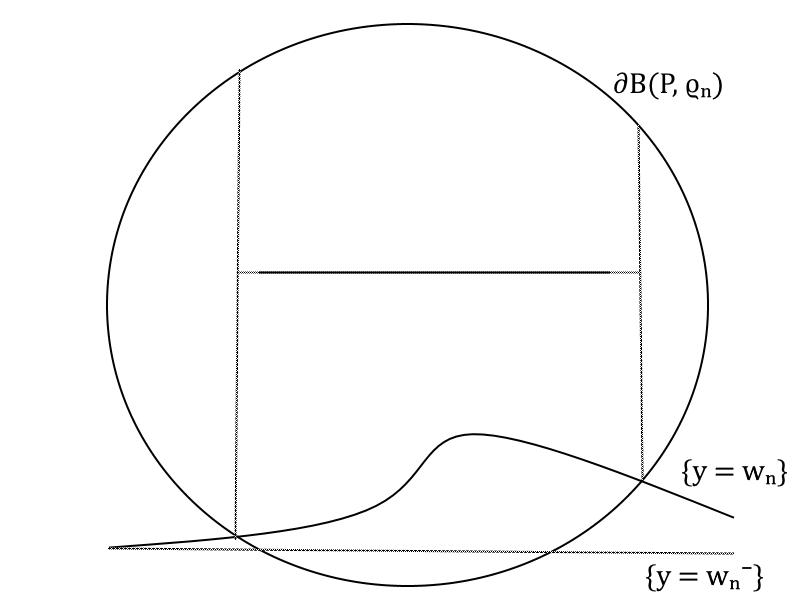
\includegraphics[width=\linewidth]{set to graph.png}
% \end{subfigure}
% \begin{subfigure}[b]{0.4\linewidth}
% 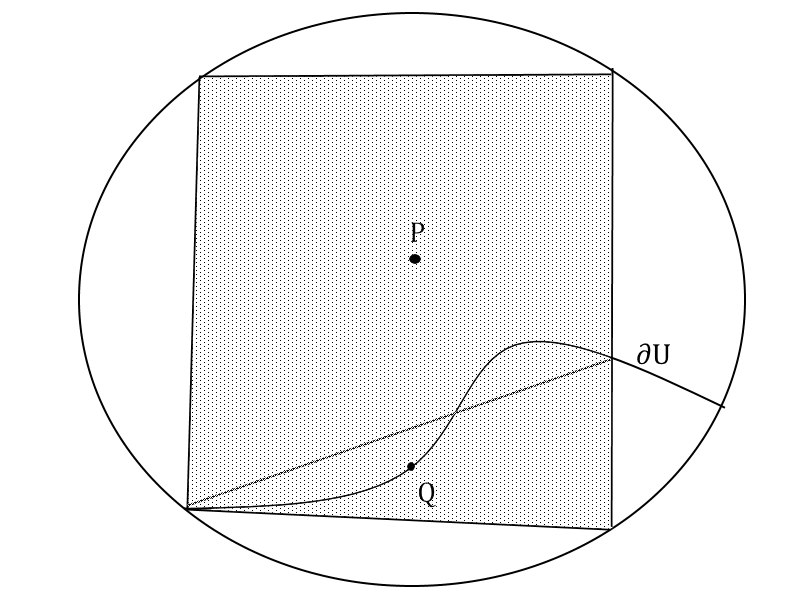
\includegraphics[width=\linewidth]{set to graph 2.png}
% \end{subfigure}
% \caption{The proof of Lemma \ref{rep as a good graph} (left) and the closely related Lemma \ref{Miranda44} (right). On the left, the dashed line through the center is $D_n^-$ and the darker line lying over it is $B_{\varpi_n}$. Notice that $B_{\varpi_n}$ is chosen to be $\Subset D_n^-$ and to be a ball centered on $P$, while $D_n^-$ is slightly off-center. On the right, the shaded region is the cylinder $I_\varpi$, and the shaded line is the graph of the minimizer $v$. The amount by which $\partial U$ fails to be a minimizer in $B(P, \rho)$ is bounded from below by its failure to equal the graph of $v$ in $I_\varpi$.}
% \label{set to graph pics}
% \end{figure}

% \begin{lemma}
% Suppose that $\partial U \cap A$ is the graph of some $C^1$ function $w$ such that $P = (0, w(0)) \in A$ and $||\dif w||_{C^0} \leq c_1$, and $\Omega := \{x \in \RR^{d - 1}: (x, w(x)) \in A\}$. Then
% \begin{equation}\label{excess vs averagers}
% \Exc_{P, A} U = \int_\Omega \Lagrange(w, \dif w) - \Lagrange(w, \avg_\rho \dif w) + O((\diam A)^{d + 1}).
% \end{equation}
% \end{lemma}
% \begin{proof}
% This is immediate from (\ref{dGL same traces concl 2}), refnoneccentric dimension, and the expansion (\ref{expand metric}) applied to $\star 1$.
% \end{proof}

We write, for $R \in M$,
$$\psi_R := \dif x^1_R \wedge \cdots \wedge \dif x^{d - 1}_R.$$

\begin{lemma}[de Giorgi lemma, $C^1$ case]\label{Miranda44}
Let $\beta, \rho > 0$, $\rho \ll_{c_1, d} |K|^{-1}$ and $\beta \lesssim_{c_0, d} 1$, and let $U$ be a set of $C^1$ perimeter in $B(P, \rho)$, such that $\Exc_\rho (U, P) \leq \beta$. Assume that $B(P, \rho)$ is contractible and there exists $Q \in B(P, \rho)$ such that
\begin{align}
\star(\normal_U \wedge \psi_Q) &\geq (1 - o(c_1^2)) |\psi_Q|, \label{Miranda44 normal hyp} \\
|\partial^* U \cap B(P, \rho)| &\leq \eta(U, B(P, \rho)) + c_1 \beta. \label{Miranda44 minimality hyp}
\end{align}
Then
\begin{equation}\label{Miranda44 concl}
\Exc_{\alpha \rho} (U, P) \leq (\alpha^{d + 1} + Cc_0) \beta + C|K|\rho^{d + 1}.
\end{equation}
\end{lemma}
\begin{proof}
Throughout this proof we assume that $\partial U \cap B(P, \alpha \rho)$ is nonempty.
If not, then (\ref{Miranda44 concl}) is vacuous since then $\Exc_{\alpha \rho} (U, P) = 0$.
For $R \in M$, let $x^\mu_R := x^\mu \circ (\Phi^R)^{-1}$.

\begin{claim}
There exists a unique $\tilde Q \in B(P, \rho)$ such that
$$\{\tilde Q\} := \partial U \cap \{x^1_Q = x^2_Q = \cdots = x^{d - 1}_Q = 0\}.$$
\end{claim}
\begin{proof}[Proof of claim]
By Lemma \ref{rep as a good graph} and (\ref{Miranda44 normal hyp}), there exists $\tilde \varpi > 0$ such that
$$\tilde \Gamma := \partial U \cap \{(x^1_Q)^2 + \cdots + (x^{d - 1}_Q)^2 < \tilde \varpi^2\}$$
is the graph of a function with respect to $(x^\mu_Q)$. In particular, any vertical line $\{(x^i_Q) = \text{const}\}$ intersects $\tilde \Gamma$ at a single point.
\end{proof}

Let $\tilde x^\mu := x^\mu_{\tilde Q}$ and $\tilde \psi := \psi_{\tilde Q}$.
Up to a gauge transformation $\chi: M \to \SpOrth(TM)$ such that $\chi^Q = \id$, we may assume that $\Phi^{\tilde Q} \circ (\Phi^Q)^{-1}$ maps the unique geodesic containing $Q, \tilde Q$ into itself, and hence $\tilde \psi = \psi + O(|K| \rho)$.
Since $\chi^Q = \id$, $\chi$ preserves the one hypothesis of this lemma which is not gauge-invariant, namely (\ref{Miranda44 normal hyp}).
By (\ref{Miranda44 normal hyp}), if $\rho/|K|$ is small depending on $c_1$,
$$\star(\normal \wedge \tilde \psi) \geq (1 - o(c_1^2)) |\tilde \psi|.$$
Therefore by Lemma \ref{rep as a good graph}, there exist $V, \Omega \subset \RR^d$ satisfying (\ref{rep as a good graph set nests}), and $w: \Omega \to \RR$ such that $||\dif w||_{C^0} \leq c_1$, and the graph of $w$ with respect to $(\tilde x^\mu)$ is
$$\Gamma := \partial U \cap \{\tilde x \in \Omega\}.$$
By definition of $\tilde Q$, $w(0) = 0$.

Let $\varpi$ be the radius of $(\alpha - c_0) V$ and 
$$I_r := \{(\tilde x, \tilde y) \in B(P, \rho): |\tilde x| < r\}.$$
By (\ref{translation invariance}) and (\ref{approximate monotone}),
$$\tilde \beta := \Exc_{I_\varpi} (U, \tilde Q) \leq \Exc_{B(P, \rho)} (U, \tilde Q) + C|K| \rho^{d + 1} \leq \beta + 2C|K| \rho^{d + 1}.$$
Replacing $\tilde \beta$ with $\max(\tilde \beta, \beta)$ as necessary, we see from (\ref{Miranda44 minimality hyp}) that
$$|\partial^* U \cap I_\varpi| \leq \eta(U, I_\varpi) + c_1 \tilde \beta.$$
To apply Lemma \ref{Miranda43} we need to relate the excess to the Plateau energy:

\begin{claim}
For $r \leq \rho$,
$$\int_{B_r} \Lagrange(w, \dif w) - \Lagrange(w, \avg_r \dif w) = e^{O(c_0)} \Exc_{B(P, r)} (U, \tilde Q) + O(|K| \rho^{d + 1}).$$
\end{claim}
\begin{proof}[Proof of claim]
By (\ref{compare Lagrangians}) we may replace $\Lagrange(w, \dif w) - \Lagrange(w, \avg_r \dif w)$ with $\Japan{\dif w} - \Japan{\avg_\rho \dif w}$.
On the other hand, in the definition of the excess we may replace the Hodge star with its euclidean counterpart.
Then this claim is proven on \cite[pg83]{Giusti77} if $\beta \lesssim_{c_0} 1$.
\end{proof}

Replacing $\tilde \beta$ with $e^{O(c_0)} \tilde \beta$ we have by Lemma \ref{Miranda43}, the claim, (\ref{translation invariance}), and (\ref{approximate monotone}) that 
\begin{align*}
\Exc_{B(P, \alpha \rho)} (U, P) &\leq \Exc_{B(P, \alpha \rho)} (U, \tilde Q) + C|K| \rho^{d + 1} \leq \Exc_{I_{\varpi/(\alpha - c_0)}} (U, \tilde Q) + C|K| \rho^{d + 1}\\
&\leq \left[\frac{1}{(\alpha + c_0)^{d + 1}} + c_0\right] \tilde \beta + C|K| \rho^{d + 1} \leq \left[\frac{1}{\alpha^{d + 1}} + Cc_0\right] \tilde \beta + C|K| \rho^{d + 1} \\
&\leq \left[\frac{1}{\alpha^{d + 1}} + Cc_0\right] \beta + C|K| \rho^{d + 1}. 
\qedhere 
\end{align*}
\end{proof}

%%%%%%%%%%%%%%%%%%%%%%%%%%%
\subsection{General case}
We now use a compactness argument to apply Proposition \ref{mollifier quant} and obtain the full de Giorgi lemma, an analogue of \cite[Teorema 5.7]{Miranda66}.

\begin{lemma}\label{single mollify}
There exists $c = c(d, K, c_0, c_1) > 0$ and $r = r(d, K, c_0, c_1) > 0$ such that for any ball $B(P, \rho)$ such that $\rho < r$ and any set $U$ of least perimeter in $B(P, \rho)$ such that
$$\Exc_\rho (U, P) \leq c\rho^{d - 1},$$
there exists a set $V$ of $C^1$ perimeter in $B(P, (1 - c_0)\rho)$ such that
\begin{align}
\star(\normal_V \wedge \psi_P) &\geq (1 - o(c_1^2))|\psi_P|, \label{single mollify normal}\\
|\partial V \cap B(P, (1 - c_0)\rho)| &\leq \eta(V, B(P, (1 - c_0)\rho)) + c_1 \Exc_\rho (U, P) + C|K| \rho^{d + 1}, \label{single mollify minimality}
\end{align}
and for $0 < \varpi \leq (1 - c_0)\rho$,
\begin{equation}
|\Exc_\varpi (U, P) - \Exc_\varpi (V, P)| \leq c_0 \Exc_\rho (U, P). \label{single mollify excess}
\end{equation}
\end{lemma}
\begin{proof}
If not, then there exist balls $B_n := B(P_n, \rho_n)$ and sets $U_n$ of least perimeter in $B_n$ such that
\begin{equation}\label{single mollify Excess assumption}
\Exc_{\rho_n} (U_n, P_n) \leq n^{-2} \rho_n^{d - 1},
\end{equation}
but such that for every set $V_n$ of $C^1$ perimeter in $B(P_n, (1 - c_0) \rho_n)$, at least one of (\ref{single mollify normal}), (\ref{single mollify minimality}), or (\ref{single mollify excess}) fail.
Since $M$ has constant sectional curvature we may assume that $P_n = P$ is fixed, and after applying a gauge transformation $\chi_n$ we may assume that
$$\Exc_{\rho_n} (U_n, P) = \int_{B_n} \star (|\dif 1_{U_n}| - \partial_0^P 1_{U_n}).$$
So by (\ref{single mollify Excess assumption}) and a Taylor expansion of the Hodge star,
$$\gamma_n := \rho_n^{1 - d} \int_{B(P, \rho_n)} |\psi_P| \cdot |\dif 1_{U_n}| - \dif 1_{U_n} \wedge \psi_P \leq \frac{1}{n^2}.$$
In particular $(\gamma_n) \in \ell^1$, so by Proposition \ref{mollifier quant}, for almost every $t \in (1 - c_0, 1)$ there exist sets $V_n$ of $C^1$ perimeter in $B(P, t\rho_n)$ such that (\ref{mollifier quant1}), (\ref{mollifier quant2}), (\ref{mollifier quant4}), and (\ref{mollifier quant3}) hold, but at least one of (\ref{single mollify normal}), (\ref{single mollify minimality}), or (\ref{single mollify excess}) fail.
Since $t > 1 - c_0$, we can restrict to consideration of $B(P, (1 - c_0) \rho_n)$, in which case (\ref{mollifier quant4}) implies (\ref{single mollify normal}) and (\ref{mollifier quant1}) implies (\ref{single mollify minimality}).
Therefore after taking a subsequence, (\ref{single mollify excess}) fails for every $n$ and some $\varpi$, that is,
\begin{equation}\label{single mollify Excess assumption 2}
|\Exc_\varpi (U, P) - \Exc_\varpi (V, P)| > \frac{c_0}{2} \gamma_n \rho_n^{d - 1}.
\end{equation}
Taking
$$\omega^\mu := \dif x^0 \wedge \cdots \wedge \widehat{\dif x^\mu} \wedge \cdots \wedge \dif x^{d - 1},$$
we see from (\ref{mollifier quant3}) that for some $\mu$,
$$\left|\int_{B(P, \varpi)} \star \partial_\mu (1_{U_n} - 1_{V_n})\right| \ll \rho_n^{d - 1} \gamma_n.$$
Combined with (\ref{mollifier quant2}) and (\ref{single mollify Excess assumption}) this contradicts the failure of (\ref{single mollify Excess assumption 2}).
\end{proof}

\begin{proof}[Proof of the de Giorgi lemma]
Let $c_0 \ll 2^{-(d + 1)}$ and $\alpha := 1/(2(1 - c_0))$.
By Lemma \ref{single mollify}, there exists a set $V$ with $C^1$ perimeter in $B(P, (1 - c_0)\rho)$ such that (\ref{single mollify normal}), (\ref{single mollify minimality}), and (\ref{single mollify excess}) hold.
By (\ref{single mollify excess}) and (\ref{approximate monotone}), for $\beta := \Exc_{B(P, \rho)} U$,
\begin{align*}
\Exc_{(1 - c_0) \rho} (V, P) &\leq \Exc_{(1 - c_0) \rho} (U, P) + c_0 \Exc_\rho (U, P) + C|K| \rho^{d + 1} \leq e^{c_0} \Exc_\rho (U, P) + C |K| \rho^{d + 1} \\
&\leq e^{c_0} \beta + C |K| \rho^{d + 1} =: \beta'.
\end{align*}
So by Lemma \ref{Miranda44} and our choice of $\alpha$,
\begin{align*}
\Exc_{\rho/2} (V, P) &\leq (2^{-(d + 1)} (1 - c_0)^{-(d + 1)} + Cc_0) \beta' + C |K| \rho^{d + 1} \\
&\leq ((1 + (d + 2) c_0) 2^{-(d + 1)} + Cc_0) \beta + C |K| \rho^{d + 1} \\
&\leq (2^{-(d + 1)} + Cc_0) \beta + C |K| \rho^{d + 1}.
\end{align*}
Applying (\ref{single mollify excess}) again, we obtain
$$\Exc_{\rho/2} (U, P) \leq (2^{-(d + 1)} + Cc_0) \Exc_{P, B(P, \rho)} U + C|K|\rho^{d + 1}$$
which is sufficient due to our choice of $c_0$.
\end{proof}


%%%%%%%%%%%%%%%%%%%%%%%%%%%%%%%%%%%%
\section{Applications of regularity}\label{GornySec}

\subsection{The maximum principle}\label{Max Princip}
We now prove Theorem \ref{main thm}, following \cite[\S3]{górny2017planar}. Let $u \in BV_\loc(M)$, $A_y = \partial \{u > y\}$, and $\lambda := \bigcup_{y \in \RR} A_y$.

\subsubsection{Least gradient implies minimal lamination}
Let $u$ have least gradient, and observe that $\lambda = \supp \dif u$, so $\lambda$ is closed.
The sets $\{u > y\}$ are totally ordered by $\subseteq$, so either $A_y = A_{y'}$ or $A_y \cap A_{y'} = \emptyset$.
By Proposition \ref{level sets are minimal}, $\{u > y\}$ has least perimeter, so by Theorem \ref{main lma}, $A_y$ is a disjoint union of $C^\infty$ minimal hypersurfaces.

\subsubsection{Local finiteness}
We now claim that the decomposition of $\{u > y\}$ into minimal hypersurfaces is finite in any compact subset $K$ of $M$.
If not, then there exists $P \in K \cap \overline{\partial U}$ and a sequence of connected components $(D_n)$, such that there exists $P_n \in D_n \cap K$ with $P_n \to P$.
Since $\partial^* U$ is dense in $\partial U$ we can in fact take $P_n \in D_n^* := D_n \cap \partial^* U$.
Now we take $\varepsilon > 0$ so small that $e^{-A\varepsilon^2} \geq 1/2$, and choose $N$ so large that if $n \geq N$ then $B_n := B(P_n, \varepsilon/2)$ is contained in $B := B(P, \varepsilon)$.
Thus by Proposition \ref{doubling dimension},
$$|\partial U \cap B| \geq \sum_{n=N}^\infty |D_n^* \cap B_n| \geq \sum_{n=N}^\infty \frac{\varepsilon^{d - 1}}{2^d} |\Ball^{d - 1}| = \infty,$$
which violates that $U$ has locally finite perimeter.

\subsubsection{Surfaces with boundary}
Now suppose that $\overline M$ is a surface-with-boundary.
We must show that if $\gamma_1, \gamma_2$ are two distinct geodesics in the lamination $\lambda$, then their extensions $\overline \gamma_i$ to $\overline M$ do not intersect on $\partial M$.
If they do intersect at $P \in \partial M$, then $\gamma_1, \gamma_2$ bound the same superlevel set $\{u > y\}$.
Let $Q, R$ be points on $\gamma_1, \gamma_2$ respectively which are so close to $P$ that $P, Q, R$ bound a nondegenerate, contractible geodesic triangle $T$.
By local finiteness, we may assume that no geodesics in $A_y$ pass through the interior of $T$.
Since $\{u > y\}$ has least perimeter, $v = 1_{\{u > y\}}$ has least gradient, and without loss of generality we may assume that $v = 1$ inside $T$ and $v = 0$ on the opposite sides of $\gamma_1, \gamma_2$.
Moreover $\int_M \star |\dif v|$ is the sum of lengths of geodesics in $A_y$.
If we define $\tilde v = v$ away from the interior of $T$ and $\tilde v = 0$ on $T$, then $\int_M \star |\dif \tilde v|$ is the sum of lengths of geodesics in $A_y$, but with $\overline{PQ}$ and $\overline{PR}$ replaced by $\overline{QR}$.
So by the triangle inequality and the fact that $T$ is nondegenerate,
$$\int_M \star |\dif \tilde v| < \int_M \star |\dif v|,$$
yet by construction $\tilde v$ and $v$ have the same trace (which is well-defined by Proposition \ref{traces}).
This is a contradiction since $v$ has least gradient.

\begin{figure}
\centering
\begin{subfigure}[b]{0.4\linewidth}
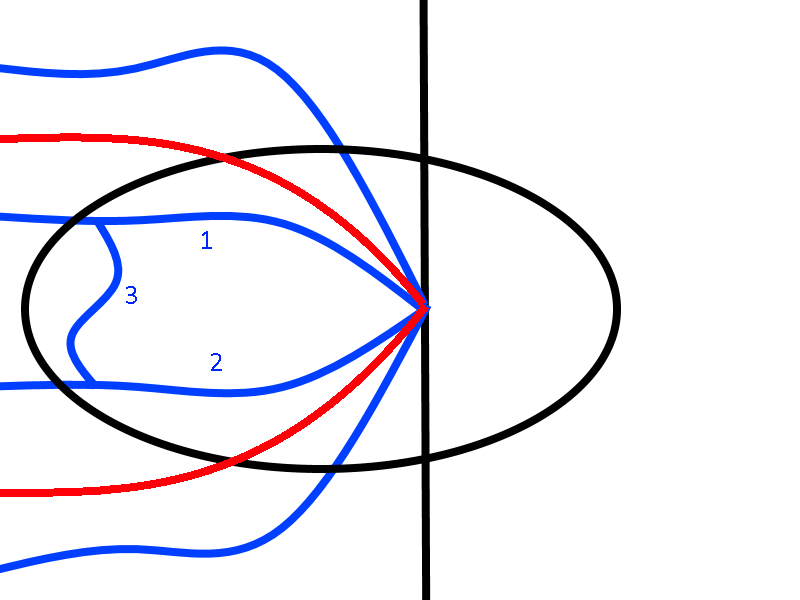
\includegraphics[width=\linewidth]{geodesic_triangle.png}
\end{subfigure}
\begin{subfigure}[b]{0.4\linewidth}
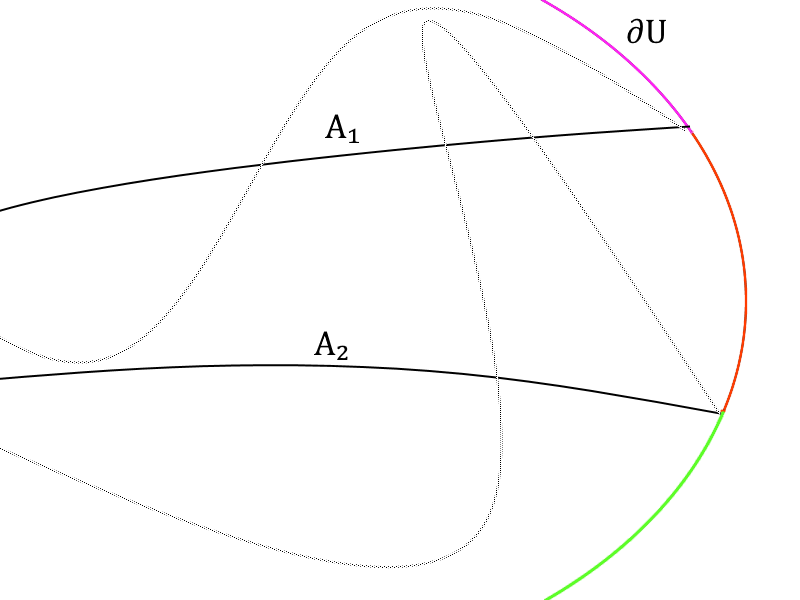
\includegraphics[width=\linewidth]{converse_max.png}
\end{subfigure}
\caption{The left picture illustrates the $d = 2$ case.
The geodesic triangle $T$ is lightly shaded, bounded by the geodesics $\gamma_1, \gamma_2, \overline{QR}$. Here $\{u > y\} = \{v > 0\}$ is shaded, and $\{\tilde v > 0\}$ is darkly shaded.
The right picture illustrates the converse to the maximum principle. The function $u$ is constant on each colored piece of $\partial U$, and its level sets $A_1, A_2$ form a geodesic lamination.
The competitor $v$ has the same trace on $\partial U$, but its level sets (the lighter curves) are not geodesics and so by the coarea formula, $u$ is smaller.}
\label{max_princip_graphs}
\end{figure}

\subsubsection{Minimal lamination implies least gradient}
Now suppose that $\lambda$ is a minimal lamination whose set of leaves is discrete, so every set $A_y$ is minimal and $y$ ranges over a discrete set $\Gamma$.
Fix $U \Subset M$ with Lipschitz boundary, let $T: BV(U) \to L^1(\partial U)$ be the trace map, and let $v$ be a competitor in $U$, thus $v \in BV(U)$ and $Tu = Tv$.
In particular, for every $y \in \Gamma$, $\{Tu \geq y\} = \{Tv \geq y\}$.

By (\ref{convergence of trace}), for any $w \in BV(U)$, $x \in \partial U$, and $z \in \RR$, $T(1_{w > z})(x)$ is the density of $\{w > z\}$ in an infinitesimal neighborhood of $x$.
Let $\varepsilon > 0$ be so small that $\{Tu > y\} = \{Tu > y - 2\varepsilon\}$, which exists since $\Gamma$ is discrete.
If $Tv(x) > y$, then the density of $\{v > y - \varepsilon/2\}$ near $x$ is $1$, so $T(1_{\{v > y - \varepsilon/2\}})(x) = 1$, so 
$$1_{\{Tu > y\}} = 1_{\{Tv > y\}} \leq T(1_{\{v > y - \varepsilon/2\}}).$$
Conversely, if $Tv(x) \leq y - \varepsilon$, then the density of $\{v > y - \varepsilon/2\}$ near $x$ is $0$. Thus 
$$T(1_{\{v > y - \varepsilon/2\}}) \leq T(1_{\{v > y - \varepsilon\}}) \leq 1_{\{Tv > y - \varepsilon\}} = 1_{\{Tu > y - \varepsilon\}} = 1_{\{Tu > y\}}.$$
The inequalities collapse and imply that $1_{\{Tu > y - \varepsilon\}} = T(1_{\{v > y - \varepsilon\}})$.
This is true for $\varepsilon$ arbitrarily small, so
$$1_{\{Tu \geq y\}} = T(1_{\{v \geq y\}}).$$
The left-hand side is $T(1_{\{u > y\}})$ since $u$ is locally constant away from $\lambda$ (since $\Gamma$ is discrete).
Therefore $A_y$ and $1_{\{v \geq y\}}$ are competitors, thus since $A_y$ is minimal, 
\begin{equation}\label{laminationwise least gradient}
|A_y \cap U| \leq |\partial^* \{v \geq y\} \cap U|.
\end{equation}
We now integrate both sides of (\ref{laminationwise least gradient}) against $\dif y$ and apply the coarea formula, Proposition \ref{coarea formula}, to see that
$$\int_U \star |\dif u| = \int_{-\infty}^\infty |A_y \cap U| \dif y \leq \int_{-\infty}^\infty |\partial^* \{v \geq y\} \cap U| \dif y = \int_U \star |\dif v|,$$
    implying that $u$ has least gradient.

\subsection{G\'orny decomposition}
We next prove Theorem \ref{Gorny regularity}, following \cite[\S3]{górny2017planar}.
We begin by decomposing functions of least gradient into sections using the following proposition.
It essentially appears for contractible sets in \cite[pg10-11]{górny2017planar} but we found it more elegant to reprove the result in a way which better shows the importance of the topology.

\begin{definition}
Let $u \in BV(M)$. The \dfn{jumpset} of $u$ is the set $J_u$ of $x \in M$ such that there exists $\normal \in T_x'M$ and $u(x-) < u(x+) \in \RR$ such that 
\begin{align*}
\lim_{r \to 0} \dashint_{B(x, r) \cap (\exp_x)_* \{v \in T_xM: (\normal, v) > 0\}} \star |u - u(x+)|  & = 0, \\
\lim_{r \to 0} \dashint_{B(x, r) \cap (\exp_x)_* \{v \in T_xM: (\normal, v) < 0\}} \star |u - u(x-)|  & = 0.
\end{align*}
\end{definition}

\begin{proposition}\label{existence of jump graphs}
Let $u \in BV(M)$ satisfy:
\begin{enumerate}
\item $u$ only has jump discontinuities,
\item the jumpset of $u$ is a lamination $\lambda$ of $M$ with countably many leaves,
\item each leaf of $\lambda$ is the locally finite union of submanifolds of $M$ without boundary, and
\item the traces of $u$ along each leaf $N$ of $\lambda$ are constant on $N$.
\end{enumerate}
Then there exists an affine line bundle $E \to M$, which is flat with structure group $\RR$, and a section $Ju: M \to E$ such that $Ju$ is locally constant on $M \setminus \lambda$ and for each leaf $N$ of $\lambda$, the amounts that $u, Ju$ jump along $N$ are equal.
\end{proposition}
\begin{proof}
We first observe that $\pi_0(M \setminus \lambda)$ is nonempty and countable, since $\lambda$ is a countable union of null sets and so $M \setminus \lambda$ is nonempty, and since $\lambda$ only has countably many connected components.
We define a new lamination $\tilde \lambda$, as follows. Initialize $\tilde \lambda := \lambda$ and replace each leaf in $\lambda$ with its connected components.
We then adjoin further leaves to $\tilde \lambda$ so that for each $U \in \pi_0(M \setminus \tilde \lambda)$, if $\mathcal V(U)$ denotes the set of components which are adjacent to $U$, then $\overline{U \cup \bigcup_{V \in \mathcal V(U)} V}$ is contained in a simply connected subset of $M$.

We set $\{U_i: i \in I\} = \pi_0(M \setminus \tilde \lambda)$ for a countable set $I$.
We endow $I$ with the structure of a weighted directed multigraph, where the set of edges $E_{ij}$ from $i$ to $j$ is $E_{ij} := \pi_0(\partial U_i \cap \partial U_j)$ if $i \neq j$.
Thus each element of $E_{ij}$ is a leaf of $\tilde \lambda$.
We weight an edge $N \in E_{ij}$ by the amount that $u$ jumps along any curve $\gamma$ from $U_i$ to $U_j$ transverse to $N$ when $\gamma$ passes through $N$.
Note that the leaves we adjoined all have weight $0$.

We choose $x_i \in U_i$ for each $i \in I$.
We call a path $\sum_k N_k$ through $I$, where $N_k$ is an edge $i_k \to j_k$, a \dfn{boundary} if there are curves $\gamma_1, \dots, \gamma_m$, where $\gamma_k$ is a curve $x_{i_k} \to x_{j_k}$ that is transverse to $\tilde \lambda$ and passes through $N_k$ exactly once, and the homology class $[\sum_k \gamma_k]$ is zero.

\begin{claim}
The total weight of any boundary is $0$.
\end{claim}
\begin{proof}[Proof of claim]
Let $k = 1, \dots, n$, let $\gamma := \sum_k \gamma_k$ be the associated $1$-chain to a boundary $\sum_k N_k$, and let $w_k$ be the weight of $N_k$.
If we set $v$ to be $u$ on $U_{i_1}$, $u - w_1$ on $U_{i_2}$, etc., $u - \sum_{k < n} w_k$ on $U_{i_n}$, then $v$ is continuous away from $N_{i_n}$ where it has a jump discontinuity of size $\sum_k w_k$.
Then $\int_\gamma \dif v = 0$ but also $\int_\gamma \dif v = \sum_k w_k$.
\end{proof}

Let $P_{ij}$ be the set of paths $i \to j$.
It follows that if $p, q \in P_{ij}$ are \dfn{homologous} in the sense that $p - q$ is a boundary, then $p, q$ have the same total weight.
On the other hand, if $i, j$ are adjacent, then for $N, N' \in E_{ij}$ and $\gamma, \gamma': x_i \to x_j$ which are respectively transverse to $N, N'$ and do not leave $\overline U_i \cup \overline U_j$, $[\gamma - \gamma'] = 0$, so $N, N'$ are homologous and hence have the same weight.

We now define $V_i$ to be the interior of $\overline U_i \cup \bigcup_{E_{ij} \neq \emptyset} \overline U_j$.
Then $(V_i)$ is an open cover of $M$.
For $x \in V_i \setminus \tilde \lambda$, let $j(x)$ be such that $x \in U_{j(x)}$, and let $Ju_i(x)$ be the weight of some (and hence any) edge in $E_{ij(x)}$ if $j(x) \neq i$, or $Ju_i(x) = 0$ if $j(x) = i$.
Then $Ju_i$ is well-defined, locally constant, and jumps by the same amount along each leaf of $\tilde \lambda$ in $V_i$ as $u$.
Moreover, on $V_i \cap V_j$, $Ju_i - Ju_j = Ju_i(x_j)$ which is constant.
Now the desired bundle $E$ exists with flat trivializations $V_i$ and transition functions $s_{ij} := Ju_i(x_j)$.
If $V_i \cap V_j \cap V_k$ is nonempty, then it is contained in a simply connected set and so $s_{ik} = s_{ij} + s_{jk}$.
\end{proof}

\begin{figure}
\centering
\begin{subfigure}[b]{0.4\linewidth}
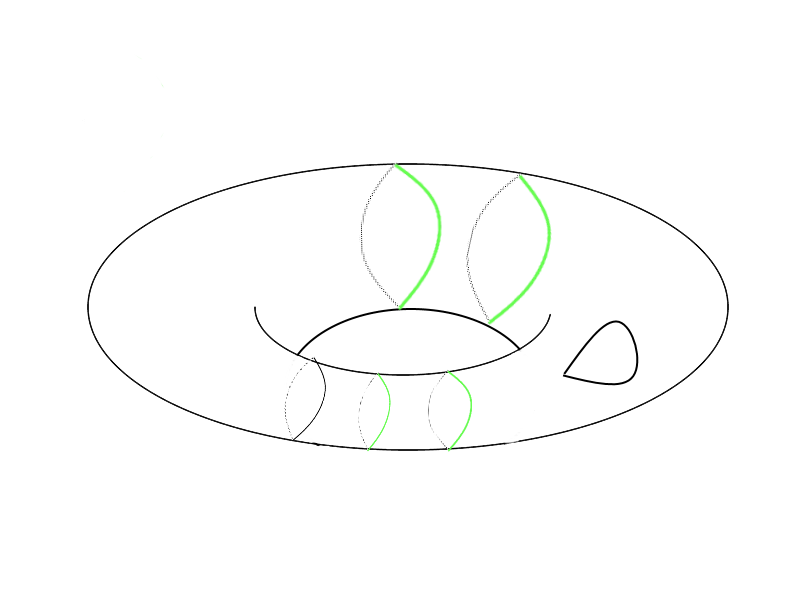
\includegraphics[width=\linewidth]{sample torus.png}
\end{subfigure}
\begin{subfigure}[b]{0.4\linewidth}
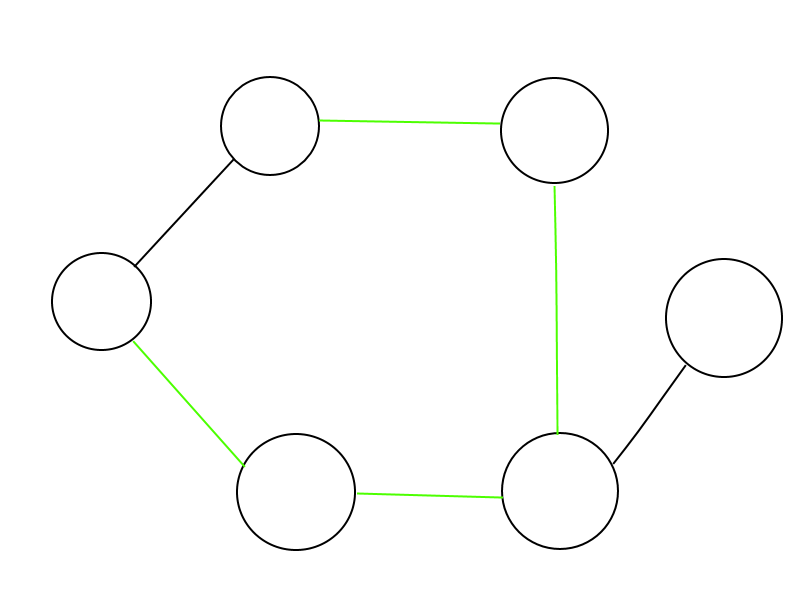
\includegraphics[width=\linewidth]{torus graph.png}
\end{subfigure}
\caption{The proof of Proposition \ref{existence of jump graphs} in case $M = \mathbf T^2$ and $u$ has two jump discontinuities, along each of the black loops. Note that we have to adjoin green leaves in order to ensure the simple connectedness condition, and that if we were to retract the green edges of the graph, then there would be a vertex of $I$ with a self-loop.}
\label{torus graphs}
\end{figure}

\begin{proof}[Proof of Theorem \ref{Gorny regularity}]
Let $u$ be a function of least gradient on $M$.
Let
\begin{align*}
\hat u(x) &:= \inf\left\{t \in \RR: \lim_{r \to 0} \frac{|\{u \leq t\} \cap B(x, r)|}{|B(x, r)|} = 1\right\},\\
\check u(x) &:= \sup\left\{t \in \RR: \lim_{r \to 0} \frac{|\{u \geq t\} \cap B(x, r)|}{|B(x, r)|} = 1\right\},
\end{align*}
and let $J_u$ be the jumpset of $u$.
Reasoning identically to the proof of \cite[Proposition 3.9]{górny2017planar} we see that $J_u = \{\hat u \neq \check u\}$.
By \cite[Theorem 4.1]{HakkarainenKorteLahtiShanmugalingam+2015}, it follows that $u := \check u$ only has jump discontinuities.
Moreover, $J_u$ is a sublamination of the minimal lamination $\lambda$ furnished by the maximum principle, and along each connected component of any leaf in $J_u$, the trace of $u$ from each side is constant along $N$.
So by Proposition \ref{existence of jump graphs}, there exists a unique (up to isomorphism) decomposition $u = u_j - u_c$ into sections $u_j, u_c: M \to E$, where $E$ is a flat affine line bundle with struture group $\RR$, such that $u_j$ is locally constant on $M \setminus \lambda$, $u_j$ has the same jumpset, with the same traces on each leaf, as $u$, and $u_c$ has no jump discontinuties.
Reasoning identically to \cite[pg11]{górny2017planar} we see that $u_j, u_c$ have locally least gradient.
Repeating the reasoning from the start of this proof and using the fact that $u_c$ has no jump discontinuities, it follows that $u_c$ is continuous.
\end{proof}

%%%%%%%%%%%%%%%%%%%%%%
% \subsection{Numerical analysis of minimal laminations}\label{numerics}
% The maximum principle, when combined with recent work of Loisel \cite{Loisel20}, furnishes a large class of minimal laminations which are inexpensive to numerically compute.
% For simplicity, we consider the model case that $M$ is a closed space form such that $\pi_1(M)$ is nonzero, but the results of this section can be easily extended to other manifolds $M$ of constant sectional curvature.
% We give an algorithm for constructing minimal laminations in $M$, and provide the results of some numerical experiments used to construct some examples of minimal laminations in three dimensions.

% We begin by recalling Loisel's theorem \cite[Theorem 1]{Loisel20} on the numerical analysis of the $p$-Laplacian in the limiting case $p = 1$.

% \begin{definition}
% By the \dfn{PL finite element space} associated to a triangulation $\mathcal T$ of a polytope $\overline \Omega \subset \RR^d$ we mean the space of all continuous functions $u: \overline \Omega \to \RR$ whose restrictions $u|T$, $T \in \mathcal T$, are linear.
% We equip a PL finite element space with the norm inherited from $W^{1, 1}(\Omega) \subset BV(\Omega)$.
% By a \dfn{PL trace} we mean a continuous function $f: \partial \Omega \to \RR$ such that if $T \in \mathcal T$ intersects $\partial \Omega$, then $f|T \cap \partial \Omega$ is linear.
% \end{definition} 

% Following \cite[\S3.2]{Loisel20}, we identify any PL trace $f$ with its \dfn{discrete harmonic prolongation}, that is, the minimizer $v$ of $\int_\Omega \star |\dif v|^2$ in the PL finite element space subject to $v|\partial \Omega = f$.
% Thus $||v||_V \lesssim ||f||_{L^1(\partial \Omega)}$.

% \begin{theorem}[Loisel]
% Let $\Omega$ be a polytope in $\RR^d$ and let $\mathcal T$ be a triangulation of $\Omega$ with quasiuniformity parameter $\lesssim 1$.
% Let $V$ be the PL finite element space associated to $\mathcal T$ and let $f$ be a PL trace.
% Let $u \in V$ minimize $\int_\Omega \star |\dif u|$ subject to the constraints $u \in V$, $u|\partial \Omega = f$.
% Then the barrier method of \cite[\S2.3]{Loisel20} returns $u$ with runtime $\lesssim |\mathcal T|^{1/2} \log (|\mathcal T|\Japan{||f||_V})$.
% \end{theorem}

% The same argument shows the above result holds when the Hodge star is not necessarily the euclidean Hodge star.
% TODO: Confirm this.

% Let $M$ be a closed space form, let $\xi \in H^1(M, \ZZ)$ be a cohomology class, and let $u: M \to \Sph^1$ be a map of least gradient such that $\xi = [\dif u]$.
% Then we associate to $\xi$ the minimal lamination induced by $u$.
% Note that $u$ may not be unique.

% TODO: How are all these things stored in memory?

% TODO: The algorithm. Turn $\xi$ into Dirichlet data, compute a tolerance, run Loisel's algorithm, and then use the fact that every leaf runs through the boundary to get the leaves.

% \begin{proposition}\label{application to Loisel}
% Let $M$ be a closed space form, and let $\xi \in H^1(M, \ZZ)$.
% Then Algorithm TODO returns the minimal lamination associated to $\xi$.
% Moreover, the runtime is TODO.
% \end{proposition}

% TODO: Do some numerical experiments, show what minimal laminations in a fundamental polytope in $\Hyp^3$ or $\Sph^3$ look like

%%%%%%%%%%%%%%%%

\appendix 
\section{Geometric computations}\label{geometric computations}
Throughout this appendix, let $M = K^{-2}\Sph^d$ or $M = |K|^{-2}\Hyp^d$, for some sectional curvature $K$, expressed using stereographic projection (for $M = \Sph^d$) or the Poincar\'e ball model (for $M = \Hyp^d$).
We write $|P|$ for the euclidean distance of $P$ to $O$, and $P - Q$ for the vector obtained from affine subtraction in $\RR^d$.

\begin{lemma}\label{Coxeter estimate}
Let $P \in M$ and let $\gamma$ be the unique geodesic through $O, P$.
Let $\Phi^P: M \to M$ be the unique oriented isometry of $M$ such that $\Phi^P(P) = O$ and $\Phi^P$ maps $\gamma$ into itself.
Then on $T_QM$, $Q \in M$,
$$|\dif \Phi^P - \id| \lesssim |K|(|P|^2 + |P| \cdot |Q|).$$
\end{lemma}
\begin{proof}
We prove this in case $K = -1$, in which case we have 
$$\varphi(Q) := (\Phi^P)^{-1}(Q) = \frac{(1 - |P|^2)Q + (|Q|^2 + 2P \cdot Q + 1)P}{|P|^2 |Q|^2 + 2P \cdot Q + 1}$$
by \cite[(4.5.5)]{ratcliffe2006foundations}.
The cited proof only relies on the fact that the isometry group of $M$ is Coxeter and generated by spherical inversions, so we can adapt it to the case $K = +1$ as well. TODO: Write out the details for $K = +1$.
The case of general $K$ follows by a scaling argument.

We now compute 
\begin{align*}
\dif \varphi &= (1 - |P|^2) \dif \frac{Q}{|P|^2|Q|^2 + 2P \cdot Q + 1} + P \otimes \dif \frac{|Q|^2 + 2P \cdot Q + 1}{|P|^2 |Q|^2 + 2P\cdot Q + 1} \\
&= \frac{1 - |P|^2}{|P|^2 |Q|^2 + 2 P \cdot Q + 1} \id - \frac{1 - |P|^2}{(|P|^2 |Q|^2 + 2P \cdot Q + 1)^2}(2|P|^2Q^{\otimes 2} + 2P \otimes Q) \\
&\qquad + \frac{2Q \otimes P + 2P^{\otimes 2}}{|P|^2 |Q|^2 + 2P \cdot Q + 1} - \frac{|Q|^2 + 2P \cdot Q + 1}{(|P|^2 |Q|^2 + 2P \cdot Q + 1)^2} (2Q \otimes P + 2P^{\otimes 2}) \\
&= \id + O(|P|^2 + |P| \cdot |Q|). 
\end{align*}
Inverting $\dif \varphi$ using a Neumann series completes the proof.
\end{proof}

\begin{lemma}\label{convex balls}
Let $B \subset M$ be a ball such that $O \in B$.
If $\diam B \lesssim |K|$, then $B$ appears convex in coordinates.
\end{lemma}
\begin{proof}
By rescaling we may assume that $|K| = 2$, so that 
$$\dist(P, Q) = \mathrm{arsinh} \sqrt{\delta(P, Q)}, \qquad \delta(P, Q) := \frac{|P - Q|^2}{(1 \pm |P|^2)(1 \pm |Q|^2)}$$
where the $\pm$ is the sign of $K$ and if $K = -1$ then $|P|, |Q| < 1$.
In particular, if $B = B(Q, r)$, $\delta := \delta(\cdot, Q)$, and $\delta_* := \sinh^2 r$, then $\partial B$ is cut out by the equation $\delta = \delta_*$.
Therefore $B$ appears convex in coordinates if its second fundamental form $\Two = \nabla(\dif \delta/|\dif \delta|)$ is positive-definite (where the second fundamental form, Levi-Civita connection, and cometric are all euclidean).
For $Q$ fixed, $\dif \delta$ is proportional to 
$$\xi := (1 \pm |P|^2)^{-1} \left[\left(1 + \frac{|P - Q|^2}{1 \pm |P|^2}\right)P - Q\right] = P - Q + O(|P|^2 + |Q|^2),$$
and $\nabla \xi = \id + O(|P| + |Q|)$.
In particular,
\begin{align*}
\Two &= \nabla\frac{\xi}{|\xi|} = \frac{\nabla \xi}{|\xi|} - \frac{\xi \otimes \nabla|\xi|}{|\xi|^2} \\
&= |\xi|^{-1} \left[\nabla \xi - \frac{\xi \otimes \tr(\xi \otimes \nabla \xi)}{|\xi|}\right] \\
&= |\xi|^{-1} [\id + O(|\xi| + |P| + |Q|)] = |\xi|^{-1} [\id + O(r)]
\end{align*}
which is positive-definite for $r \ll 1$.
\end{proof}

\printbibliography

\end{document}
